\section{Mô hình Khuếch tán (Diffusion Models)}
\label{sec:diffusion_models}

Trong khi GANs thống trị lĩnh vực sinh ảnh trong nhiều năm, chúng vẫn tồn tại những thách thức cố hữu về sự ổn định trong huấn luyện và hiện tượng sụp đổ mode. Vào khoảng năm 2020, một họ mô hình sinh mới, lấy cảm hứng từ nhiệt động lực học, đã nổi lên và nhanh chóng chiếm lĩnh vị trí dẫn đầu: \textbf{Mô hình Khuếch tán (Diffusion Models)}. Với khả năng tạo ra những hình ảnh có chất lượng và sự đa dạng vượt trội, cùng với quá trình huấn luyện ổn định hơn, các mô hình khuếch tán đã mở ra một cuộc cách mạng sáng tạo mới, đặc biệt trong lĩnh vực tạo ảnh từ văn bản.

\subsection{Lý thuyết Cơ bản: DDPM và Quá trình Khuếch tán}
\label{subsec:diffusion_theory}

\subsubsection{Tại sao cần Diffusion Models?}
\label{subsubsec:diffusion_motivation}

Trước khi đi vào cơ chế hoạt động, hãy hiểu tại sao diffusion models ra đời. Hai họ mô hình sinh phổ biến trước đó --- VAE và GAN --- đều có những giới hạn cố hữu:

\textbf{VAE} tối ưu một cận dưới của log-likelihood (ELBO), đây là mục tiêu thanh lịch về mặt lý thuyết nhưng thực tế dẫn đến hai vấn đề: (1) ảnh sinh ra thường bị \textit{mờ} do hàm reconstruction loss MSE bình quân hóa các pixel, và (2) cân bằng giữa reconstruction term và KL divergence term đòi hỏi tinh chỉnh hyperparameter cẩn thận.

\textbf{GAN} sinh ảnh sắc nét ấn tượng nhưng training nổi tiếng là bất ổn. Ba vấn đề chính: (1) \textit{Training instability} --- nếu Discriminator quá mạnh hoặc quá yếu so với Generator, training diverge; (2) \textit{Mode collapse} --- Generator chỉ học sinh một vài mẫu, bỏ qua phần còn lại của phân phối dữ liệu; (3) \textit{Khó đánh giá} --- không có metric đơn giản nào đánh giá cả chất lượng lẫn đa dạng.

\textbf{Diffusion models} giải quyết những vấn đề này bằng cách tiếp cận hoàn toàn khác: thay vì huấn luyện hai mạng cạnh tranh nhau hay ép encoder vào một phân phối cụ thể, diffusion models \textit{học cách đảo ngược một quá trình phá hủy dữ liệu được định nghĩa toán học rõ ràng}. Kết quả là training ổn định (loss là MSE đơn giản), ảnh chất lượng cao, và phân phối đầy đủ không bị mode collapse.

\subsubsection{Ý tưởng Cốt lõi: Noise và Denoise}
\label{subsubsec:core_idea}

\textbf{Trực giác.} Hãy tưởng tượng bạn nhỏ một giọt mực vào cốc nước trong. Giọt mực ban đầu có hình dạng rõ ràng; dần dần nó lan ra và hòa tan hoàn toàn sau vài phút --- đây là \textit{khuếch tán (diffusion)}: từ trật tự đến hỗn loạn. Nếu ta có thể học cách đảo ngược quá trình này, ta có thể tạo ra dữ liệu mới từ nhiễu ngẫu nhiên.

Diffusion models hoạt động theo hai quá trình đối lập:

\begin{enumerate}
    \item \textbf{Forward process (quá trình thuận)}: Lấy ảnh sạch $\mathbf{x}_0$, từ từ thêm nhiễu Gaussian qua $T$ bước rời rạc ($T = 1000$ trong DDPM gốc). Sau $T$ bước, ảnh biến thành nhiễu Gaussian thuần túy $\mathbf{x}_T \approx \mathcal{N}(\mathbf{0}, \mathbf{I})$. Quá trình này \textit{cố định, không cần học} --- nó chỉ là một công thức toán học xác định trước.
    \item \textbf{Reverse process (quá trình ngược)}: Huấn luyện mạng nơ-ron để đảo ngược từng bước --- nhận $\mathbf{x}_t$ (ảnh nhiễu), xuất ra $\mathbf{x}_{t-1}$ (ảnh ít nhiễu hơn). Lặp lại $T$ bước bắt đầu từ nhiễu thuần túy $\mathbf{x}_T$ để sinh ra ảnh mới $\mathbf{x}_0$.
\end{enumerate}

\begin{center}
    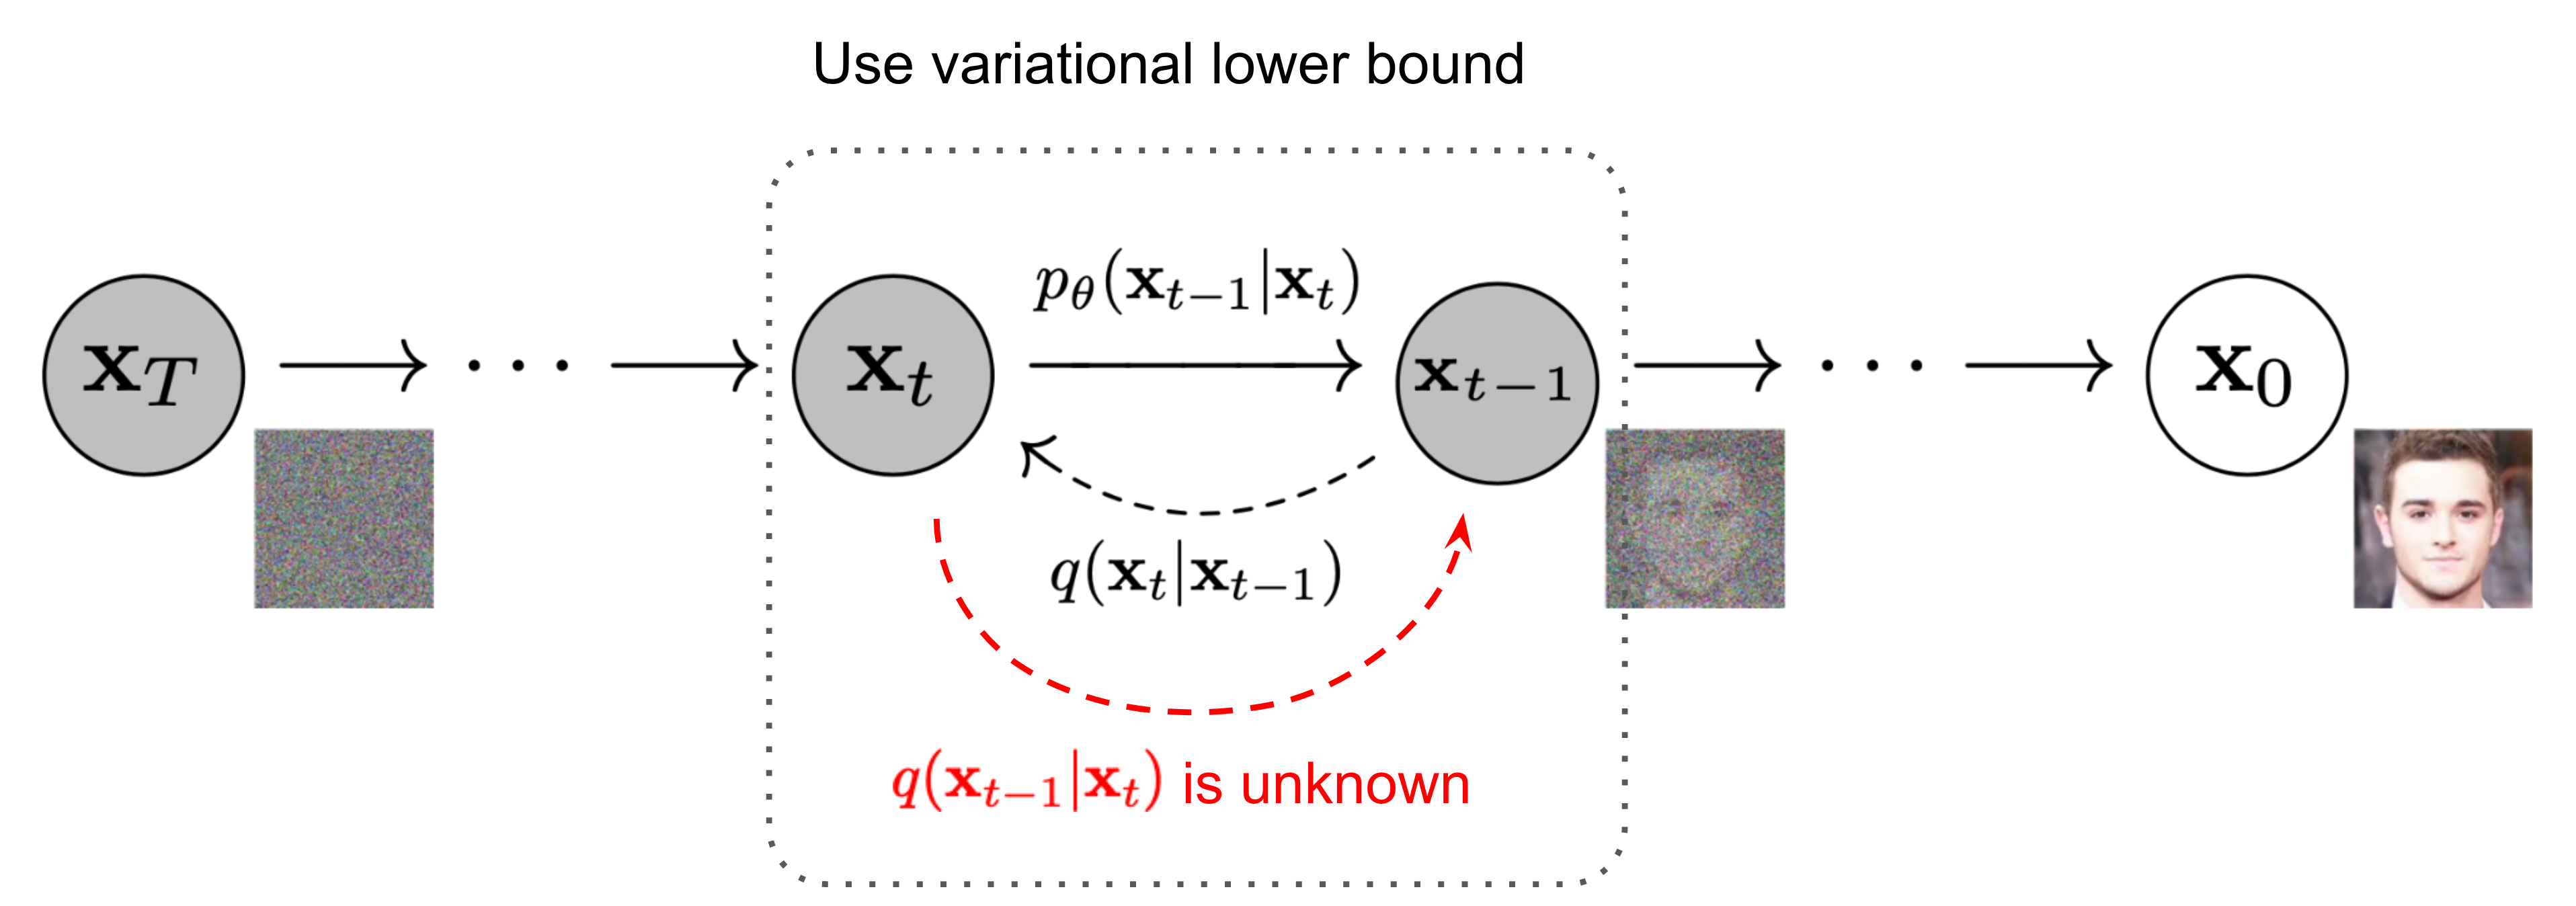
\includegraphics[width=0.98\textwidth]{images/ddpm_diffusion_process.png}
    \captionof{figure}{Hai quá trình của Diffusion Model. \textbf{Forward process} (trái $\to$ phải): thêm nhiễu dần dần qua $T$ bước. \textbf{Reverse process} (phải $\to$ trái): mạng U-Net khử nhiễu từng bước, từ $\mathbf{x}_T$ trở về $\mathbf{x}_0$.}
    \label{fig:diffusion_two_process}
\end{center}

\subsubsection{Khung Xác suất của DDPM}
\label{subsubsec:ddpm_framework}

\textbf{DDPM} \cite{Ho2020} (Ho et al., 2020) hình thức hóa ý tưởng trên trong ngôn ngữ xác suất. Mục tiêu của generative modeling là học phân phối $q(\mathbf{x}_0)$ của dữ liệu thật để có thể sinh mẫu mới từ một mô hình xấp xỉ $p_\theta(\mathbf{x}_0)$.

\begin{mdframed}[style=infobox]
\textbf{Bảng ký hiệu --- đọc trước khi vào công thức}

\begin{tabular}{lp{10cm}}
$\mathbf{x}_0$ & Ảnh gốc sạch. \textbf{In đậm} vì là vector/tensor, không phải số vô hướng. \\
$\mathbf{x}_t$ & Ảnh sau $t$ bước thêm nhiễu ($t = 1, \ldots, T$). \\
$q(\cdot)$ & Phân phối \textit{thật}, cố định (forward process). \\
$p_\theta(\cdot)$ & Phân phối được \textit{học} bởi mạng tham số $\theta$ (reverse process). \\
$\mathcal{N}(\mathbf{x};\,\boldsymbol{\mu},\,\sigma^2\mathbf{I})$ & Phân phối Gaussian với mean $\boldsymbol{\mu}$ và variance $\sigma^2$ ở mỗi chiều. \\
$\mathcal{N}(\mathbf{0},\mathbf{I})$ & Gaussian chuẩn: mean = 0, variance = 1 mỗi chiều. \\
$\boldsymbol{\epsilon} \sim \mathcal{N}(\mathbf{0},\mathbf{I})$ & Lấy mẫu vector nhiễu ngẫu nhiên cùng kích thước với ảnh. \\
$\beta_t \in (0,1)$ & Lượng nhiễu thêm vào bước $t$ (hyperparameter, không học). \\
$\alpha_t = 1 - \beta_t$ & Tỷ lệ tín hiệu giữ lại ở bước $t$. \\
$\bar{\alpha}_t = \prod_{i=1}^t \alpha_i$ & Tích lũy: tỷ lệ tín hiệu gốc còn lại sau \textit{tất cả} $t$ bước. \\
$\mathbb{E}[\cdot]$ & Kỳ vọng (trung bình theo phân phối). \\
$\theta$ & Tham số của mạng nơ-ron (trọng số cần học). \\
$\boldsymbol{\epsilon}_\theta(\mathbf{x}_t, t)$ & Mạng dự đoán nhiễu từ ảnh nhiễu $\mathbf{x}_t$ và timestep $t$. \\
\end{tabular}
\end{mdframed}

\subsubsection{Forward Process: Markov Chain Thêm Nhiễu}
\label{subsubsec:forward_process}

Forward process được định nghĩa là một \textbf{Markov chain} --- chuỗi biến ngẫu nhiên trong đó $\mathbf{x}_t$ chỉ phụ thuộc vào $\mathbf{x}_{t-1}$, không phụ thuộc lịch sử trước đó:
\[
    q(\mathbf{x}_t \mid \mathbf{x}_{t-1}, \mathbf{x}_{t-2}, \ldots, \mathbf{x}_0) = q(\mathbf{x}_t \mid \mathbf{x}_{t-1})
\]
Toàn bộ quá trình từ $\mathbf{x}_0$ đến $\mathbf{x}_T$ viết gọn là:
\begin{equation}
    q(\mathbf{x}_{1:T} \mid \mathbf{x}_0) = \prod_{t=1}^T q(\mathbf{x}_t \mid \mathbf{x}_{t-1})
\end{equation}
\textbf{Đọc công thức:} ``Xác suất của toàn bộ chuỗi $\mathbf{x}_1, \mathbf{x}_2, \ldots, \mathbf{x}_T$ bằng tích xác suất của từng bước chuyển tiếp.'' Ký hiệu $\mathbf{x}_{1:T}$ là viết tắt cho $\mathbf{x}_1, \mathbf{x}_2, \ldots, \mathbf{x}_T$.

\textbf{Xác suất chuyển tiếp một bước.}
Mỗi bước chuyển tiếp là một Gaussian: thêm nhiễu có phương sai $\beta_t$, đồng thời co tín hiệu lại một chút:
\begin{equation}
    q(\mathbf{x}_t \mid \mathbf{x}_{t-1}) = \mathcal{N}\!\left(\mathbf{x}_t;\; \underbrace{\sqrt{1-\beta_t}}_{\text{scale down tín hiệu}}\,\mathbf{x}_{t-1},\;\; \underbrace{\beta_t\,\mathbf{I}}_{\text{phương sai nhiễu}}\right)
    \label{eq:forward_step}
\end{equation}

Dùng reparameterization trick, ta viết tương đương: nếu $\boldsymbol{\epsilon}_{t-1} \sim \mathcal{N}(\mathbf{0},\mathbf{I})$, thì:
\[
    \mathbf{x}_t = \sqrt{\alpha_t}\,\mathbf{x}_{t-1} + \sqrt{1-\alpha_t}\,\boldsymbol{\epsilon}_{t-1}, \qquad \alpha_t = 1 - \beta_t
\]
\textbf{Giải thích:} $\sqrt{\alpha_t}$ ($\approx 0.999$) làm tín hiệu giảm nhẹ; $\sqrt{1-\alpha_t}$ ($\approx 0.03$) là độ lớn của nhiễu thêm vào. Vì $\beta_t$ nhỏ, sự thay đổi mỗi bước rất nhỏ nhưng sau 1000 bước tích lũy thì ảnh gốc bị phá hủy hoàn toàn.

\textbf{Lịch trình nhiễu (Noise Schedule).}
Dãy $\{\beta_t\}_{t=1}^T$ là \textit{hyperparameter được chọn trước}, không phải tham số học. Hai lịch trình phổ biến:

\textit{Linear schedule} (DDPM gốc): $\beta_t$ tăng tuyến tính từ $\beta_\text{start} = 10^{-4}$ đến $\beta_\text{end} = 0.02$:
\[
    \beta_t = \beta_\text{start} + (t-1) \cdot \frac{\beta_\text{end} - \beta_\text{start}}{T-1}, \qquad t = 1, \ldots, T
\]

\textit{Cosine schedule} (Improved DDPM, 2021): được thiết kế qua $\bar{\alpha}_t$ để thay đổi chậm hơn ở đầu và cuối:
\[
    \bar{\alpha}_t = \frac{f(t)}{f(0)}, \quad f(t) = \cos^2\!\left(\frac{t/T + s}{1+s} \cdot \frac{\pi}{2}\right)
\]
trong đó $s = 0.008$ là offset nhỏ. Từ $\bar{\alpha}_t$ suy ngược ra $\beta_t = 1 - \bar{\alpha}_t/\bar{\alpha}_{t-1}$. Cosine schedule tránh phá hủy thông tin quá nhanh ở các bước đầu, thường cho kết quả tốt hơn linear.

\textbf{Công thức vàng: Nhảy thẳng từ $\mathbf{x}_0$ đến $\mathbf{x}_t$.}
Nếu phải chạy 1000 vòng lặp để tạo $\mathbf{x}_t$ từ $\mathbf{x}_0$, training sẽ cực kỳ chậm. Nhờ tính chất của phân phối Gaussian --- \textit{tổng của hai Gaussian độc lập là một Gaussian khác} --- ta có thể chứng minh công thức closed-form:

\begin{equation}
    \boxed{\mathbf{x}_t = \sqrt{\bar{\alpha}_t}\,\mathbf{x}_0 + \sqrt{1-\bar{\alpha}_t}\,\boldsymbol{\epsilon}, \qquad \boldsymbol{\epsilon} \sim \mathcal{N}(\mathbf{0},\mathbf{I})}
    \label{eq:ddpm_forward_direct}
\end{equation}

Tương đương, phân phối có điều kiện là:
\begin{equation}
    q(\mathbf{x}_t \mid \mathbf{x}_0) = \mathcal{N}\!\left(\mathbf{x}_t;\; \sqrt{\bar{\alpha}_t}\,\mathbf{x}_0,\; (1-\bar{\alpha}_t)\mathbf{I}\right)
\end{equation}

\textbf{Dẫn xuất công thức (\ref{eq:ddpm_forward_direct}).}
Thay thế $\mathbf{x}_{t-1}$ bằng biểu thức theo $\mathbf{x}_{t-2}$, rồi $\mathbf{x}_{t-2}$ theo $\mathbf{x}_{t-3}$...:
\begin{align*}
\mathbf{x}_t &= \sqrt{\alpha_t}\,\mathbf{x}_{t-1} + \sqrt{1-\alpha_t}\,\boldsymbol{\epsilon}_{t-1} \\
&= \sqrt{\alpha_t}\!\left(\sqrt{\alpha_{t-1}}\,\mathbf{x}_{t-2} + \sqrt{1-\alpha_{t-1}}\,\boldsymbol{\epsilon}_{t-2}\right) + \sqrt{1-\alpha_t}\,\boldsymbol{\epsilon}_{t-1} \\
&= \sqrt{\alpha_t\alpha_{t-1}}\,\mathbf{x}_{t-2} + \underbrace{\sqrt{\alpha_t(1-\alpha_{t-1})}\,\boldsymbol{\epsilon}_{t-2} + \sqrt{1-\alpha_t}\,\boldsymbol{\epsilon}_{t-1}}_{\text{hai Gaussian độc lập}}
\end{align*}
Hai Gaussian độc lập $Z_1 \sim \mathcal{N}(0,\sigma_1^2\mathbf{I})$ và $Z_2 \sim \mathcal{N}(0,\sigma_2^2\mathbf{I})$ khi cộng lại cho $Z_1+Z_2 \sim \mathcal{N}(0,(\sigma_1^2+\sigma_2^2)\mathbf{I})$. Áp dụng: phương sai tổng của phần nhiễu là $\alpha_t(1-\alpha_{t-1}) + (1-\alpha_t) = 1 - \alpha_t\alpha_{t-1}$. Do đó:
\[
    \mathbf{x}_t = \sqrt{\alpha_t\alpha_{t-1}}\,\mathbf{x}_{t-2} + \sqrt{1-\alpha_t\alpha_{t-1}}\,\bar{\boldsymbol{\epsilon}}_{t-2}
\]
Tiếp tục đến $\mathbf{x}_0$ và dùng $\bar{\alpha}_t = \prod_{i=1}^t \alpha_i$, ta được công thức (\ref{eq:ddpm_forward_direct}).

\textbf{Ý nghĩa thực tiễn của $\bar{\alpha}_t$:}
\begin{itemize}
    \item $\sqrt{\bar{\alpha}_t}$: \textbf{signal rate} --- tỷ lệ ảnh gốc còn lại sau $t$ bước. Giảm từ 1 (khi $t=0$) về 0 (khi $t=T$).
    \item $\sqrt{1-\bar{\alpha}_t}$: \textbf{noise rate} --- tỷ lệ nhiễu. Tăng từ 0 lên 1.
    \item Khi $t$ nhỏ: $\mathbf{x}_t \approx \mathbf{x}_0$ (ảnh gần như sạch).
    \item Khi $t = T$: $\bar{\alpha}_T \approx 0$, $\mathbf{x}_T \approx \boldsymbol{\epsilon} \sim \mathcal{N}(\mathbf{0},\mathbf{I})$ (nhiễu thuần túy).
\end{itemize}

\subsubsection{Reverse Process: Học cách Khử Nhiễu}
\label{subsubsec:reverse_process}

Mục tiêu là học quá trình ngược: từ $\mathbf{x}_T$ (nhiễu) dần dần tái tạo $\mathbf{x}_0$ (ảnh sạch). Toàn bộ reverse process viết là:
\begin{equation}
    p_\theta(\mathbf{x}_{0:T}) = p(\mathbf{x}_T) \prod_{t=1}^T p_\theta(\mathbf{x}_{t-1} \mid \mathbf{x}_t)
    \label{eq:reverse_full}
\end{equation}
\textbf{Đọc công thức (\ref{eq:reverse_full}):} ``Xác suất của toàn bộ quỹ đạo ngược bằng xác suất điểm khởi đầu $p(\mathbf{x}_T) = \mathcal{N}(\mathbf{0},\mathbf{I})$ nhân với tích xác suất của từng bước khử nhiễu $p_\theta(\mathbf{x}_{t-1}|\mathbf{x}_t)$ được học bởi mạng nơ-ron.''

\textbf{Tại sao $q(\mathbf{x}_{t-1}|\mathbf{x}_t)$ không tính được trực tiếp?}
Theo Bayes: $q(\mathbf{x}_{t-1}|\mathbf{x}_t) \propto q(\mathbf{x}_t|\mathbf{x}_{t-1}) \cdot q(\mathbf{x}_{t-1})$. Để tính $q(\mathbf{x}_{t-1})$ cần tích phân qua toàn bộ phân phối dữ liệu $q(\mathbf{x}_0)$ --- chính là thứ ta đang cố học.

Tuy nhiên, nếu biết thêm $\mathbf{x}_0$, phân phối ngược \textit{có thể tính được}:
\begin{equation}
    q(\mathbf{x}_{t-1} \mid \mathbf{x}_t, \mathbf{x}_0) = \mathcal{N}\!\left(\mathbf{x}_{t-1};\; \tilde{\boldsymbol{\mu}}_t(\mathbf{x}_t, \mathbf{x}_0),\; \tilde{\beta}_t \mathbf{I}\right)
    \label{eq:reverse_posterior}
\end{equation}
trong đó:
\[
    \tilde{\boldsymbol{\mu}}_t(\mathbf{x}_t, \mathbf{x}_0) = \frac{\sqrt{\bar{\alpha}_{t-1}}\,\beta_t}{1-\bar{\alpha}_t}\,\mathbf{x}_0 + \frac{\sqrt{\alpha_t}(1-\bar{\alpha}_{t-1})}{1-\bar{\alpha}_t}\,\mathbf{x}_t, \qquad \tilde{\beta}_t = \frac{(1-\bar{\alpha}_{t-1})\,\beta_t}{1-\bar{\alpha}_t}
\]

Ý tưởng huấn luyện: \textit{dùng $q(\mathbf{x}_{t-1}|\mathbf{x}_t,\mathbf{x}_0)$ làm target trong training} (ta biết $\mathbf{x}_0$ khi training), rồi train $p_\theta(\mathbf{x}_{t-1}|\mathbf{x}_t)$ để xấp xỉ nó khi không có $\mathbf{x}_0$ (lúc inference).

\textbf{Mạng nơ-ron học gì --- Dự đoán nhiễu hay dự đoán ảnh?}
Thay vì học mean $\tilde{\boldsymbol{\mu}}_t$ trực tiếp (một ảnh hoàn chỉnh, khó học), DDPM thay thế $\mathbf{x}_0$ từ công thức (\ref{eq:ddpm_forward_direct}) vào:
\[
    \mathbf{x}_0 = \frac{\mathbf{x}_t - \sqrt{1-\bar{\alpha}_t}\,\boldsymbol{\epsilon}}{\sqrt{\bar{\alpha}_t}}
\]
và huấn luyện mạng $\boldsymbol{\epsilon}_\theta(\mathbf{x}_t, t)$ để \textbf{dự đoán nhiễu $\boldsymbol{\epsilon}$}. Dự đoán nhiễu đơn giản hơn vì $\boldsymbol{\epsilon} \sim \mathcal{N}(\mathbf{0},\mathbf{I})$ là phân phối chuẩn, không phụ thuộc nội dung ảnh.

\subsubsection{Kiến trúc U-Net và Time Embedding}
\label{subsubsec:unet_arch}

Mạng $\boldsymbol{\epsilon}_\theta(\mathbf{x}_t, t)$ nhận hai đầu vào: ảnh nhiễu $\mathbf{x}_t$ và timestep $t$.

\textbf{U-Net} được chọn làm kiến trúc vì: (1) giữ nguyên kích thước đầu vào-đầu ra, (2) skip connections cho phép gradient chảy thông suốt, (3) encoder học semantic high-level, decoder học spatial detail.

\textbf{Sinusoidal Time Embedding}: Timestep $t$ (một số nguyên từ 1 đến 1000) được chuyển thành vector $d$-chiều:
\[
    \text{PE}(t, 2i) = \sin\!\left(\frac{t}{10000^{2i/d}}\right), \qquad \text{PE}(t, 2i+1) = \cos\!\left(\frac{t}{10000^{2i/d}}\right)
\]
Vector này được cộng vào mỗi lớp ResNet của U-Net thông qua affine transformation học được. Nhờ đó, cùng một kiến trúc U-Net xử lý đúng cách ở mọi mức độ nhiễu $t$.

\begin{center}
    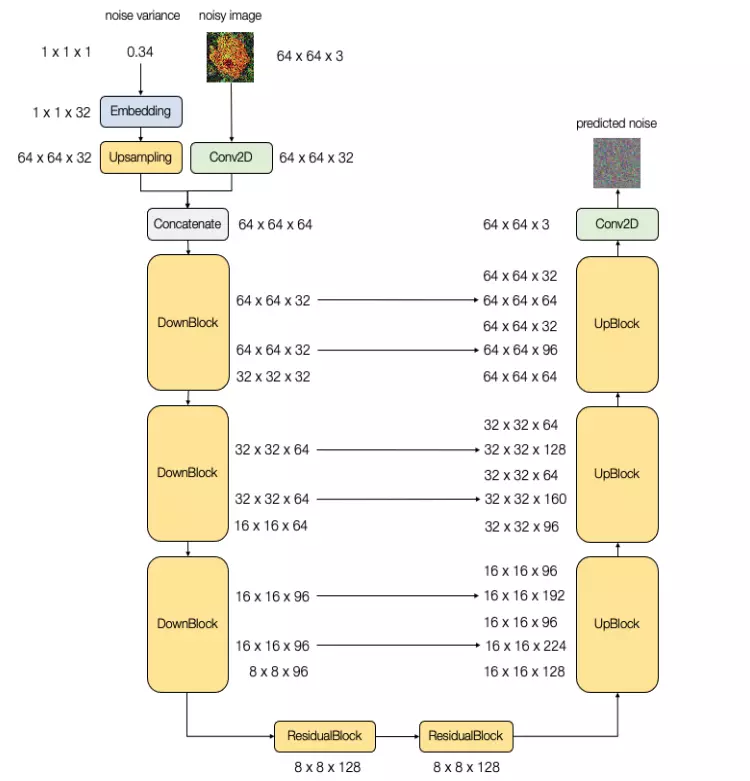
\includegraphics[width=0.85\textwidth]{images/diffusion_c890b55f.png}
    \captionof{figure}{Kiến trúc U-Net trong DDPM: ảnh nhiễu $\mathbf{x}_t$ đi qua DownBlocks (giảm độ phân giải, tăng depth), ResidualBlocks (bottleneck), và UpBlocks (khôi phục độ phân giải) với skip connections. Noise variance $\sigma_t$ được embed vào mỗi block.}
    \label{fig:unet_ddpm}
\end{center}

\begin{center}
    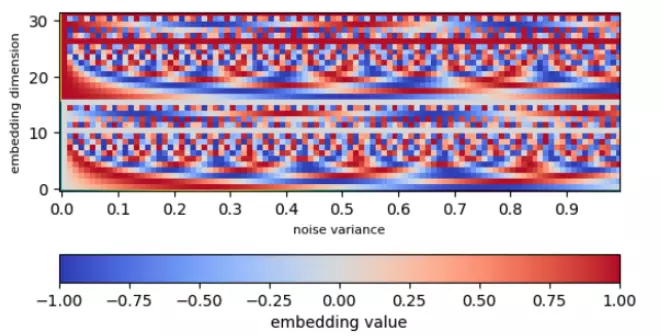
\includegraphics[width=0.85\textwidth]{images/diffusion_8c11024e.png}
    \captionof{figure}{Sinusoidal time embedding: mỗi timestep $t$ tạo ra một ``chữ ký'' vector riêng biệt (heatmap), giúp U-Net phân biệt đang xử lý bước nhiễu nào. Các bước gần nhau có embedding gần nhau; các bước xa thì khác biệt.}
    \label{fig:time_embedding}
\end{center}

\subsubsection{Hàm Mất mát: Từ ELBO đến MSE Đơn giản}
\label{subsubsec:ddpm_loss}

Mục tiêu tổng quát là tối đa hóa log-likelihood $\log p_\theta(\mathbf{x}_0)$. Do tích phân nhiều biến tiềm ẩn, ta tối ưu \textbf{Evidence Lower Bound (ELBO)}:
\[
    \log p_\theta(\mathbf{x}_0) \geq \mathcal{L}_\text{ELBO} = \mathbb{E}_q\!\left[\log p_\theta(\mathbf{x}_0|\mathbf{x}_1)\right] - D_\text{KL}(q(\mathbf{x}_T|\mathbf{x}_0)\|p(\mathbf{x}_T)) - \sum_{t=2}^T \underbrace{D_\text{KL}(q(\mathbf{x}_{t-1}|\mathbf{x}_t,\mathbf{x}_0)\|p_\theta(\mathbf{x}_{t-1}|\mathbf{x}_t))}_{\mathcal{L}_{t-1}}
\]
Sau khi khai triển và đơn giản hóa (thay $p_\theta(\mathbf{x}_{t-1}|\mathbf{x}_t)$ bằng Gaussian với mean $\boldsymbol{\mu}_\theta$ học được), mỗi term $\mathcal{L}_{t-1}$ trở thành:
\[
    \mathcal{L}_{t-1} = \mathbb{E}_q\!\left[\frac{1}{2\sigma_t^2}\left\|\tilde{\boldsymbol{\mu}}_t(\mathbf{x}_t,\mathbf{x}_0) - \boldsymbol{\mu}_\theta(\mathbf{x}_t,t)\right\|^2\right]
\]

DDPM thay $\boldsymbol{\mu}_\theta$ bằng biểu thức dưới dạng $\boldsymbol{\epsilon}_\theta$ (dự đoán nhiễu thay vì dự đoán mean), và bỏ các hệ số weighting $1/(2\sigma_t^2)$ theo kinh nghiệm thực nghiệm, thu được hàm mất mát đơn giản hóa:

\begin{equation}
    \mathcal{L}_{\text{simple}} = \mathbb{E}_{t \sim \mathcal{U}[1,T],\;\mathbf{x}_0 \sim q(\mathbf{x}_0),\;\boldsymbol{\epsilon} \sim \mathcal{N}(\mathbf{0},\mathbf{I})}
    \Bigl[\,\bigl\|\boldsymbol{\epsilon} - \boldsymbol{\epsilon}_\theta\!\bigl(\underbrace{\sqrt{\bar{\alpha}_t}\,\mathbf{x}_0 + \sqrt{1-\bar{\alpha}_t}\,\boldsymbol{\epsilon}}_{\mathbf{x}_t},\; t\bigr)\bigr\|^2\,\Bigr]
    \label{eq:ddpm_loss}
\end{equation}

\textbf{Giải thích từng thành phần:}
\begin{itemize}
    \item $t \sim \mathcal{U}[1,T]$: chọn ngẫu nhiên đều một bước trong $[1,T]$.
    \item $\mathbf{x}_0 \sim q(\mathbf{x}_0)$: lấy một ảnh từ dataset huấn luyện.
    \item $\boldsymbol{\epsilon} \sim \mathcal{N}(\mathbf{0},\mathbf{I})$: lấy mẫu nhiễu ngẫu nhiên.
    \item $\sqrt{\bar{\alpha}_t}\,\mathbf{x}_0 + \sqrt{1-\bar{\alpha}_t}\,\boldsymbol{\epsilon}$: đây là $\mathbf{x}_t$ theo công thức (\ref{eq:ddpm_forward_direct}) --- tạo ảnh nhiễu bước $t$ \textit{trực tiếp} không cần vòng lặp.
    \item $\boldsymbol{\epsilon}_\theta(\mathbf{x}_t, t)$: mạng dự đoán nhiễu.
    \item $\|\boldsymbol{\epsilon} - \boldsymbol{\epsilon}_\theta(\cdots)\|^2$: MSE giữa nhiễu thật và nhiễu dự đoán.
\end{itemize}

\subsubsection{Vòng lặp Huấn luyện và Sampling}
\label{subsubsec:ddpm_train_sample}

\textbf{Vòng lặp huấn luyện một batch:}
\begin{enumerate}
    \item Lấy batch ảnh sạch $\{\mathbf{x}_0^{(i)}\}$ từ dataset.
    \item Chọn ngẫu nhiên timestep $t^{(i)} \sim \mathcal{U}\{1,\ldots,T\}$ cho mỗi ảnh.
    \item Lấy mẫu nhiễu $\boldsymbol{\epsilon}^{(i)} \sim \mathcal{N}(\mathbf{0},\mathbf{I})$.
    \item Tính ảnh nhiễu: $\mathbf{x}_{t^{(i)}}^{(i)} = \sqrt{\bar{\alpha}_{t^{(i)}}}\,\mathbf{x}_0^{(i)} + \sqrt{1-\bar{\alpha}_{t^{(i)}}}\,\boldsymbol{\epsilon}^{(i)}$.
    \item Forward pass: $\hat{\boldsymbol{\epsilon}}^{(i)} = \boldsymbol{\epsilon}_\theta(\mathbf{x}_{t^{(i)}}^{(i)},\, t^{(i)})$.
    \item Tính loss: $\mathcal{L} = \frac{1}{B}\sum_i \|\boldsymbol{\epsilon}^{(i)} - \hat{\boldsymbol{\epsilon}}^{(i)}\|^2$.
    \item Backpropagation và cập nhật $\theta$.
\end{enumerate}

Bước 4 là lý do công thức (\ref{eq:ddpm_forward_direct}) quan trọng: mỗi ảnh trong batch được nhiễu hóa đến bước $t$ ngẫu nhiên \textit{trong một phép tính}, không cần vòng lặp $t$ bước. Điều này cho phép training song song và hiệu quả.

\textbf{Quá trình Sampling --- Sinh ảnh mới:}
\begin{enumerate}
    \item Khởi đầu: $\mathbf{x}_T \sim \mathcal{N}(\mathbf{0},\mathbf{I})$.
    \item Lặp $t = T, T-1, \ldots, 1$:
    \begin{itemize}
        \item Dự đoán nhiễu: $\hat{\boldsymbol{\epsilon}} = \boldsymbol{\epsilon}_\theta(\mathbf{x}_t, t)$.
        \item Tính $\mathbf{x}_{t-1}$:
        \[
            \mathbf{x}_{t-1} = \underbrace{\frac{1}{\sqrt{\alpha_t}}\!\left(\mathbf{x}_t - \frac{1-\alpha_t}{\sqrt{1-\bar{\alpha}_t}}\,\hat{\boldsymbol{\epsilon}}\right)}_{\text{ước tính } \tilde{\boldsymbol{\mu}}_t} + \underbrace{\sqrt{\beta_t}\,\mathbf{z}}_{\text{nhiễu ngẫu nhiên}}, \quad \mathbf{z} \sim \mathcal{N}(\mathbf{0},\mathbf{I}) \text{ (nếu }t>1\text{)}
        \]
    \end{itemize}
    \item Trả về $\mathbf{x}_0$.
\end{enumerate}

\textbf{Tại sao cộng $\sqrt{\beta_t}\,\mathbf{z}$ ở mỗi bước?} Nếu không có thành phần ngẫu nhiên này, sampling là một ODE deterministic --- mỗi lần từ cùng $\mathbf{x}_T$ sẽ cho ra cùng một ảnh $\mathbf{x}_0$. Thêm nhiễu nhỏ làm sampling trở thành SDE stochastic --- mỗi lần cho ra ảnh khác nhau, đảm bảo tính đa dạng.

\begin{center}
    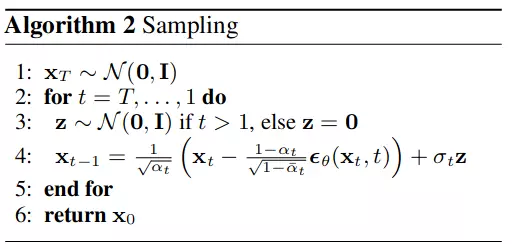
\includegraphics[width=0.65\textwidth]{images/diffusion_868fa263.png}
    \captionof{figure}{Algorithm 2 (DDPM Sampling): khởi đầu từ $\mathbf{x}_T \sim \mathcal{N}(\mathbf{0},\mathbf{I})$, lặp ngược từ $T$ về 1 sử dụng $\boldsymbol{\epsilon}_\theta$, trả về $\mathbf{x}_0$ là ảnh sinh ra.}
    \label{fig:ddpm_sampling}
\end{center}

\begin{mdframed}[style=infobox]
\textbf{DDPM so với GAN và VAE}

\begin{tabular}{lccc}
\hline
\textbf{Tiêu chí} & \textbf{VAE} & \textbf{GAN} & \textbf{DDPM} \\
\hline
Chất lượng ảnh & Trung bình (mờ) & Cao & Cao \\
Training ổn định & Tốt & Khó, bất ổn & Tốt \\
Mode collapse & Không & Thường xảy ra & Không \\
Log-likelihood & Tường minh (ELBO) & Không & Xấp xỉ (ELBO) \\
Tốc độ sampling & Nhanh ($O(1)$) & Nhanh ($O(1)$) & Chậm ($O(T)$) \\
Điều kiện hóa & Dễ & Trung bình & Dễ (CFG) \\
\hline
\end{tabular}

\medskip
\textbf{Nhược điểm chính của DDPM}: sinh ảnh cần 1000 bước forward pass qua U-Net, tức là 1000 lần chậm hơn GAN. DDIM (2020) giải quyết bằng cách bỏ yếu tố ngẫu nhiên, giảm xuống còn 50 bước. DDPM thuần túy cũng không có điều hướng --- phần tiếp theo giải quyết vấn đề này.
\end{mdframed}

\subsection{Conditional Generation: Hướng dẫn Diffusion Model Sinh ảnh theo Yêu cầu}
\label{subsec:conditional_diffusion}

DDPM thuần túy sinh ảnh ngẫu nhiên --- không có gì kiểm soát đầu ra. Để biến diffusion model thành công cụ thực dụng (``sinh ảnh mèo ngồi trên sofa đỏ''), cần một cơ chế bơm thông tin điều kiện vào quá trình denoising. Có một khái niệm nền tảng cần hiểu trước.

\textbf{Score function --- Hướng dẫn từ phân phối.}
Trong thế giới score-based models, người ta định nghĩa \textbf{score function} của một phân phối $p(\mathbf{x})$ là gradient của log-likelihood:
\[
    \mathbf{s}(\mathbf{x}) = \nabla_{\mathbf{x}} \log p(\mathbf{x})
\]
Ý nghĩa trực quan: score function tại điểm $\mathbf{x}$ trỏ về \textit{hướng tăng mật độ xác suất} --- tức là hướng làm cho $\mathbf{x}$ trông ``giống dữ liệu thật hơn''. Điều thú vị là mạng $\boldsymbol{\epsilon}_\theta$ trong DDPM thực ra đang học \textit{score function tại từng bước nhiễu} $t$:
\[
    \boldsymbol{\epsilon}_\theta(\mathbf{x}_t, t) \propto -\nabla_{\mathbf{x}_t} \log q(\mathbf{x}_t)
\]
Tức là DDPM học ``hướng nào làm cho $\mathbf{x}_t$ trở về dữ liệu thật hơn'' tại mỗi mức nhiễu --- đây chính là lý do nó khử nhiễu được.

\subsubsection{Classifier Guidance (2021) --- Mượn mắt của Classifier}
\label{subsubsec:classifier_guidance}

Dhariwal và Nichol \cite{Dhariwal2021} đặt câu hỏi: nếu ta muốn sinh ảnh thuộc lớp $y$ cụ thể (ví dụ: ``chó Golden Retriever''), làm thế nào để ``hướng'' quá trình denoising về phía lớp đó?

\textbf{Nền tảng toán học --- Quy tắc Bayes cho score.}
Ta muốn sample từ phân phối có điều kiện $p(\mathbf{x}_t \mid y)$. Bằng quy tắc Bayes:
\[
    p(\mathbf{x}_t \mid y) = \frac{p(y \mid \mathbf{x}_t)\, p(\mathbf{x}_t)}{p(y)}
\]
Lấy log gradient theo $\mathbf{x}_t$ (bỏ $p(y)$ vì không phụ thuộc $\mathbf{x}_t$):
\[
    \underbrace{\nabla_{\mathbf{x}_t} \log p(\mathbf{x}_t \mid y)}_{\text{score có điều kiện}} = \underbrace{\nabla_{\mathbf{x}_t} \log p(\mathbf{x}_t)}_{\text{score không điều kiện}} + \underbrace{\nabla_{\mathbf{x}_t} \log p(y \mid \mathbf{x}_t)}_{\text{gradient của classifier}}
\]
\textbf{Đọc công thức này như sau:} ``Hướng về phía dữ liệu-có-điều-kiện = hướng về phía dữ liệu-chung + hướng làm cho classifier nhận đúng nhãn $y$.'' Đây là một đồng nhất thức xác suất rất tự nhiên.

\textbf{Tích hợp vào denoising.}
Classifier Guidance thêm gradient của classifier vào noise prediction:
\begin{equation}
    \hat{\boldsymbol{\epsilon}} = \underbrace{\boldsymbol{\epsilon}_\theta(\mathbf{x}_t, t)}_{\text{unconditional}} - \underbrace{\sqrt{1-\bar{\alpha}_t} \cdot w \cdot \nabla_{\mathbf{x}_t} \log f_\phi(y \mid \mathbf{x}_t)}_{\text{hướng về lớp } y}
\end{equation}

\begin{itemize}
    \item $f_\phi(y \mid \mathbf{x}_t)$: classifier được huấn luyện \textit{riêng} trên ảnh nhiễu ở các mức $t$ khác nhau. Classifier thông thường train trên ảnh sạch sẽ không hoạt động vì $\mathbf{x}_t$ với $t$ lớn trông rất khác ảnh sạch.
    \item $\nabla_{\mathbf{x}_t} \log f_\phi(y \mid \mathbf{x}_t)$: gradient của log-probability theo nhãn $y$, trỏ về hướng làm ảnh ``trông giống lớp $y$ hơn'' theo mắt classifier.
    \item $w > 1$: khuếch đại lực kéo về phía $y$. Giá trị lớn → ảnh rất đặc trưng cho lớp $y$ nhưng ít đa dạng.
    \item Dấu trừ: vì $\boldsymbol{\epsilon}$ trỏ về phía nhiễu (ngược chiều score), nên trừ đi gradient classifier tương đương cộng thêm score.
\end{itemize}

\textbf{Giới hạn của Classifier Guidance:}
\begin{itemize}
    \item Phải train thêm một classifier riêng trên ảnh nhiễu --- tốn công, phức tạp pipeline.
    \item Classifier thông thường có thể ``gian lận'' --- tìm đặc trưng artifact để phân loại đúng thay vì đặc trưng ngữ nghĩa thực sự, dẫn đến gradient không đáng tin cậy.
    \item Chỉ hỗ trợ điều kiện dạng nhãn lớp (phân loại), khó mở rộng sang text hay điều kiện phức tạp.
\end{itemize}

\subsubsection{Classifier-Free Guidance --- CFG (2022) --- Không cần Classifier Ngoài}
\label{subsubsec:cfg}

Ho và Salimans \cite{Ho2022} đề xuất một cách tiếp cận thanh lịch hơn: \textit{thay vì dùng classifier ngoài, hãy để mô hình diffusion tự học đồng thời cả hai chế độ --- có và không có điều kiện.}

\textbf{Ý tưởng cốt lõi.}
Classifier Guidance cần $\nabla_{\mathbf{x}_t} \log p(y \mid \mathbf{x}_t)$. Nhưng theo Bayes:
\[
    \nabla_{\mathbf{x}_t} \log p(y \mid \mathbf{x}_t) = \nabla_{\mathbf{x}_t} \log p(\mathbf{x}_t \mid y) - \nabla_{\mathbf{x}_t} \log p(\mathbf{x}_t)
\]
Nếu mô hình diffusion học \textit{cả} $\boldsymbol{\epsilon}_\theta(\mathbf{x}_t, t, c)$ (có điều kiện) \textit{và} $\boldsymbol{\epsilon}_\theta(\mathbf{x}_t, t, \emptyset)$ (không điều kiện), thì ta có thể tính \textit{implicit classifier gradient} mà không cần classifier riêng!

\textbf{Training --- Conditioning Dropout.}
Cách train CFG đơn giản đến bất ngờ: dùng \textit{chính mạng diffusion đó} nhưng trong lúc training, với xác suất $p_\text{uncond}$ (thường 10--20\%), thay điều kiện $c$ bằng token rỗng $\emptyset$ (null embedding). Mô hình học:
\begin{itemize}
    \item 80--90\% thời gian: ``đây là ảnh nhiễu $\mathbf{x}_t$, điều kiện là $c$, hãy dự đoán nhiễu phù hợp với $c$''
    \item 10--20\% thời gian: ``đây là ảnh nhiễu $\mathbf{x}_t$, \textit{không có điều kiện}, hãy dự đoán nhiễu theo hướng dữ liệu tổng quát''
\end{itemize}
Một mạng duy nhất, hai ``mode'' hoạt động, được kiểm soát bởi $c$ có được cung cấp hay không.

\textbf{Inference --- Kết hợp hai dự đoán.}
Trong mỗi bước denoising, chạy U-Net \textit{hai lần} và kết hợp:
\begin{equation}
    \hat{\boldsymbol{\epsilon}} = \underbrace{\boldsymbol{\epsilon}_\theta(\mathbf{x}_t,\, t,\, \emptyset)}_{\substack{\text{unconditional prediction} \\ \text{``đi theo dữ liệu chung''}}}
    \;+\; w \cdot \Big(\underbrace{\boldsymbol{\epsilon}_\theta(\mathbf{x}_t,\, t,\, c)}_{\text{conditional}} - \underbrace{\boldsymbol{\epsilon}_\theta(\mathbf{x}_t,\, t,\, \emptyset)}_{\text{unconditional}}\Big)
    \label{eq:cfg}
\end{equation}

\textbf{Giải thích từng phần của công thức (\ref{eq:cfg}):}
\begin{itemize}
    \item $\boldsymbol{\epsilon}_\theta(\mathbf{x}_t, t, \emptyset)$: ``hướng khử nhiễu tự nhiên'' --- mô hình muốn đi theo phân phối dữ liệu chung, không bị ràng buộc bởi prompt.
    \item $\boldsymbol{\epsilon}_\theta(\mathbf{x}_t, t, c) - \boldsymbol{\epsilon}_\theta(\mathbf{x}_t, t, \emptyset)$: \textit{phần dư} giữa có-prompt và không-prompt. Đây chính là ``lực kéo bổ sung'' mà prompt tạo ra --- hướng duy nhất mà prompt tác động.
    \item $w$: khuếch đại lực kéo đó lên $w$ lần. $w=1$: không khuếch đại, bằng conditional prediction. $w > 1$: đẩy mạnh hơn theo hướng prompt.
\end{itemize}

Viết lại gọn hơn: $\hat{\boldsymbol{\epsilon}} = (1+w)\,\boldsymbol{\epsilon}_\theta(\mathbf{x}_t, t, c) - w\,\boldsymbol{\epsilon}_\theta(\mathbf{x}_t, t, \emptyset)$ --- đây là công thức bạn sẽ thấy trong mã nguồn Stable Diffusion.

\begin{center}
    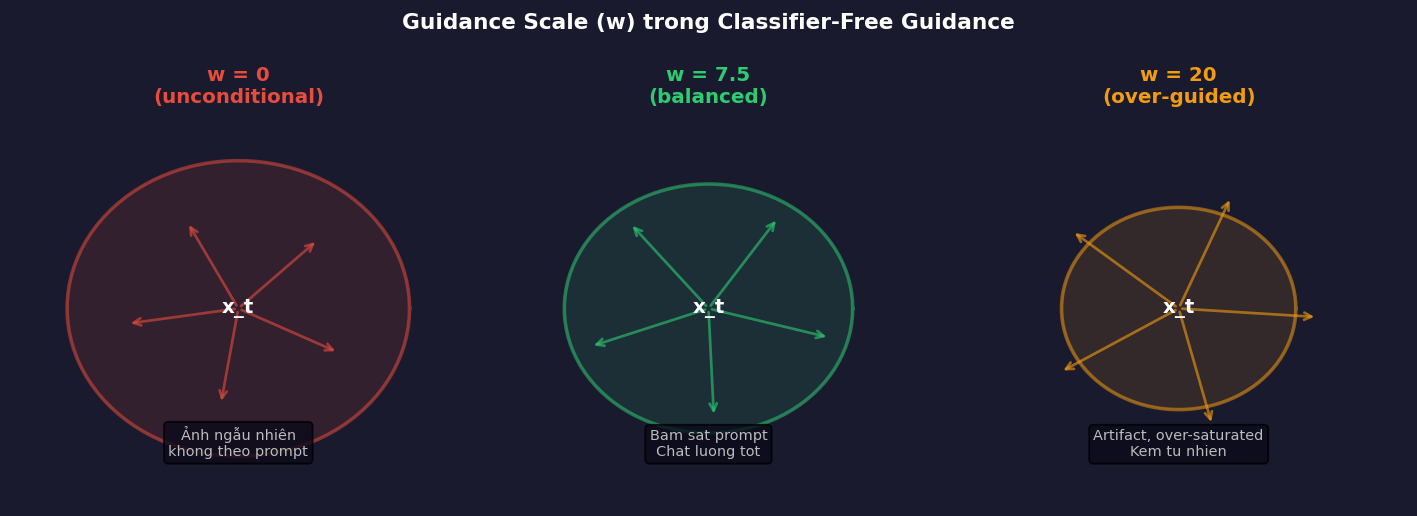
\includegraphics[width=0.90\textwidth]{images/cfg_guidance_scale.png}
    \captionof{figure}{Hiệu ứng của guidance scale $w$ trong CFG: $w=0$ sinh ảnh ngẫu nhiên không theo prompt; $w=7.5$ cân bằng giữa chất lượng và tuân theo prompt; $w=20$ ``kéo'' quá mạnh, artifact xuất hiện, màu sắc bão hòa.}
    \label{fig:cfg_scale}
\end{center}

\textbf{Negative Prompt --- Mở rộng thực tiễn của CFG.}
Một ứng dụng sáng tạo của CFG là \textbf{negative prompt}: thay vì để $\emptyset$ là điều kiện ``rỗng'', ta đặt vào đó \textit{điều ta không muốn}:
\[
    \hat{\boldsymbol{\epsilon}} = \boldsymbol{\epsilon}_\theta(\mathbf{x}_t, t, c_{\text{neg}}) + w\cdot\big(\boldsymbol{\epsilon}_\theta(\mathbf{x}_t, t, c_{\text{pos}}) - \boldsymbol{\epsilon}_\theta(\mathbf{x}_t, t, c_{\text{neg}})\big)
\]
Ví dụ: $c_\text{pos}$ = ``a beautiful portrait, high quality'' và $c_\text{neg}$ = ``blurry, low quality, distorted, watermark''. Công thức bây giờ tích cực kéo về phía $c_\text{pos}$ \textit{và} đồng thời đẩy ra xa $c_\text{neg}$.

\begin{mdframed}[style=infobox]
\textbf{Tại sao CFG tốt hơn Classifier Guidance?}

\begin{enumerate}
    \item \textbf{Không cần mô hình riêng}: chỉ cần một mạng diffusion duy nhất. Pipeline đơn giản hơn.
    \item \textbf{Gradient đáng tin cậy hơn}: classifier thông thường tìm shortcuts (artifact, texture patterns) để phân loại đúng. Mô hình diffusion buộc phải học ngữ nghĩa thực sự vì nó phải \textit{tái tạo} ảnh, không chỉ phân loại.
    \item \textbf{Hỗ trợ mọi loại điều kiện}: text, class label, ảnh tham chiếu, depth map --- chỉ cần thay $c$ tương ứng. Classifier Guidance chỉ tự nhiên với nhãn lớp phân loại.
    \item \textbf{Mở rộng tự nhiên}: negative prompt, inpainting mask, style mixing --- tất cả đều là biến thể của cùng một công thức CFG.
\end{enumerate}

CFG là kỹ thuật đứng sau thành công của DALL-E 2, Imagen (Google), và toàn bộ hệ sinh thái Stable Diffusion. Gần như mọi diffusion model text-to-image hiện đại đều dùng CFG.
\end{mdframed}

\textbf{Từ DDPM đến Stable Diffusion}: DDPM $\xrightarrow{\text{+CFG}}$ Conditional diffusion $\xrightarrow{\text{+Latent space}}$ LDM $\xrightarrow{\text{+CLIP+scale}}$ Stable Diffusion. Mỗi bước giải quyết đúng một giới hạn của bước trước.

\subsection{Latent Diffusion và Stable Diffusion: Khuếch tán trong Không gian Tiềm ẩn}
\label{subsec:latent_diffusion}

\textbf{Vấn đề căn bản của pixel-space diffusion.}
DDPM hoạt động trực tiếp trên từng pixel. Một ảnh $512 \times 512$ màu RGB có $512 \times 512 \times 3 = 786{,}432$ chiều. Mỗi bước khử nhiễu, U-Net phải xử lý tensor khổng lồ này --- và phải lặp lại 1000 lần. Huấn luyện trên hàng triệu ảnh như vậy đòi hỏi hàng trăm GPU và hàng tuần tính toán. Sinh một ảnh duy nhất mất hàng phút.

\textbf{Ý tưởng cốt lõi của LDM}: thay vì khuếch tán trong không gian pixel khổng lồ ($512 \times 512 \times 3$), hãy nén ảnh xuống một \textbf{không gian tiềm ẩn} nhỏ hơn rất nhiều ($64 \times 64 \times 4$, tức là nhỏ hơn \textbf{48 lần}), rồi chạy toàn bộ diffusion trong không gian đó. Ảnh cuối cùng được decode trở lại pixel chỉ \textit{một lần} sau khi quá trình denoising hoàn tất.

\textbf{Latent Diffusion Models (LDM)} \cite{Rombach2022} của Rombach et al. (2022) hiện thực hóa ý tưởng này qua \textbf{ba thành phần} làm việc phối hợp:

\begin{center}
    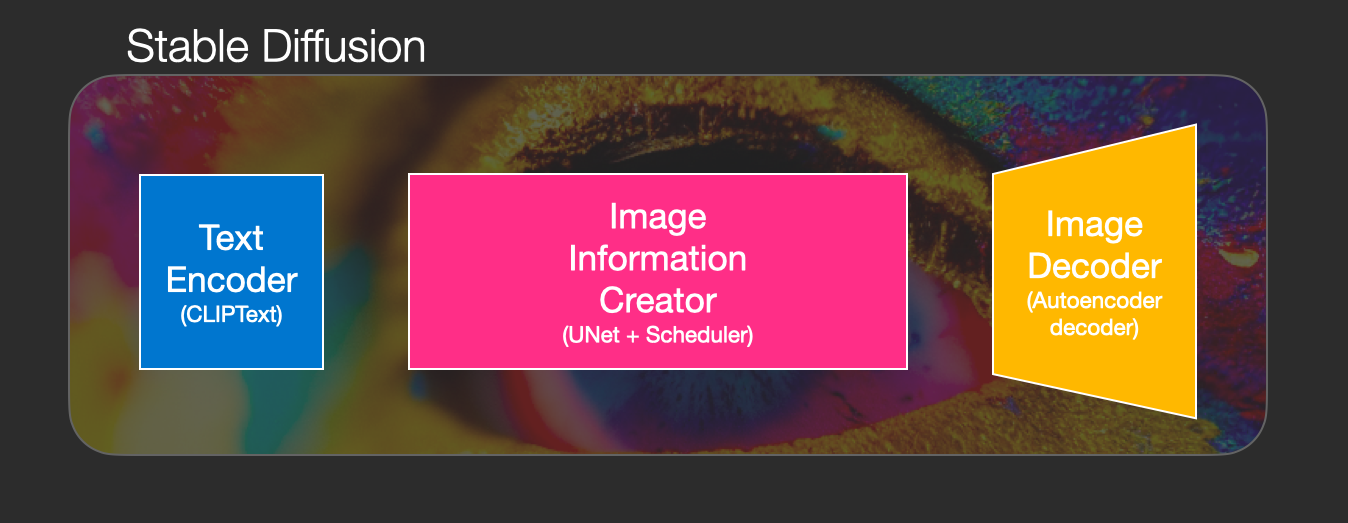
\includegraphics[width=0.90\textwidth]{images/ldm_components.png}
    \captionof{figure}{Ba thành phần của Stable Diffusion: (1) \textbf{Text Encoder} (CLIPText) chuyển prompt thành embedding, (2) \textbf{Image Information Creator} (U-Net + Scheduler) khử nhiễu lặp lại trong latent space, (3) \textbf{Image Decoder} (Autoencoder) chuyển latent thành ảnh pixel.}
    \label{fig:ldm_components}
\end{center}

\subsubsection{Thành phần 1: VAE --- Cánh cổng giữa Pixel và Latent}

\textbf{Variational Autoencoder (VAE)} là bộ phận mã hóa và giải mã không gian. Nó được huấn luyện \textit{trước} và \textit{độc lập} với phần diffusion.

\begin{center}
    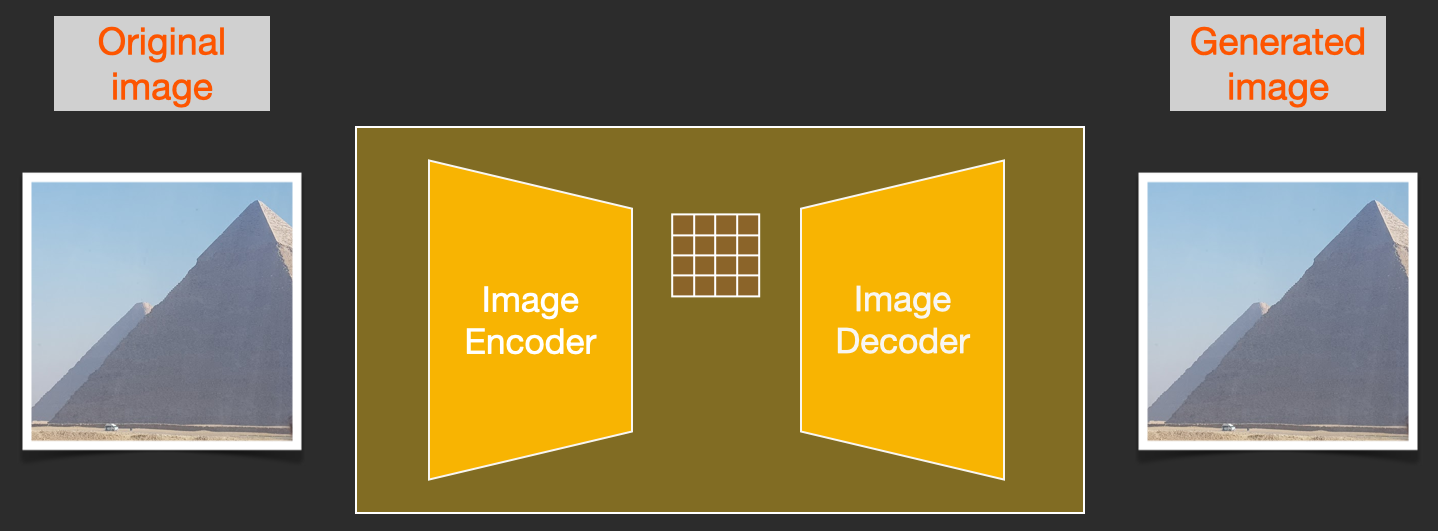
\includegraphics[width=0.88\textwidth]{images/ldm_vae.png}
    \captionof{figure}{VAE của Stable Diffusion: Image Encoder nén ảnh gốc $512\times512\times3$ thành latent $64\times64\times4$ (lưới nhỏ ở giữa), Image Decoder tái tạo ảnh từ latent. Encoder chỉ dùng khi training; trong inference chỉ cần Decoder.}
    \label{fig:ldm_vae}
\end{center}

\begin{itemize}
    \item \textbf{Encoder} $\mathcal{E}$: nhận ảnh $\mathbf{x} \in \mathbb{R}^{512 \times 512 \times 3}$, xuất ra latent $\mathbf{z} = \mathcal{E}(\mathbf{x}) \in \mathbb{R}^{64 \times 64 \times 4}$. Mỗi ``pixel'' trong latent tương ứng với một vùng $8 \times 8$ pixel gốc và mã hóa thông tin ngữ nghĩa của vùng đó.
    \item \textbf{Decoder} $\mathcal{D}$: nhận latent $\mathbf{z}$, tái tạo ảnh $\hat{\mathbf{x}} = \mathcal{D}(\mathbf{z}) \approx \mathbf{x}$. Trong inference, đây là bước cuối cùng sau khi denoising xong.
\end{itemize}

VAE được huấn luyện để nén ảnh nhưng vẫn giữ lại thông tin đủ để tái tạo chân thực. Trong inference, \textit{chỉ cần Decoder} --- Encoder không được sử dụng (không có ảnh gốc để encode).

\subsubsection{Thành phần 2: CLIP Text Encoder --- Dịch Chữ thành Số}

Để mô hình ``hiểu'' prompt văn bản, Stable Diffusion dùng \textbf{CLIP} (Contrastive Language-Image Pretraining) --- một mô hình được OpenAI huấn luyện trên 400 triệu cặp ảnh-văn bản từ internet.

CLIP học một không gian embedding chung cho cả ảnh và văn bản: những ảnh và caption mô tả cùng một thứ sẽ có embedding gần nhau. Kết quả là CLIP text encoder ``hiểu'' ngữ nghĩa sâu hơn một language model thông thường --- nó biết ``a fluffy golden retriever'' và ``a dog with curly golden fur'' đều gần nhau trong embedding space.

\textbf{Quá trình xử lý text}: Prompt được tokenize thành tối đa 77 token, mỗi token được embed thành vector 768 chiều. Kết quả là tensor $\mathbf{c} \in \mathbb{R}^{77 \times 768}$ --- ``bản tóm tắt ngữ nghĩa'' của toàn bộ prompt.

\subsubsection{Thành phần 3: U-Net trong Latent Space --- Trái tim của quá trình sinh ảnh}

U-Net trong Stable Diffusion nhận \textit{ba} đầu vào đồng thời và dự đoán nhiễu cần loại bỏ:

\begin{center}
    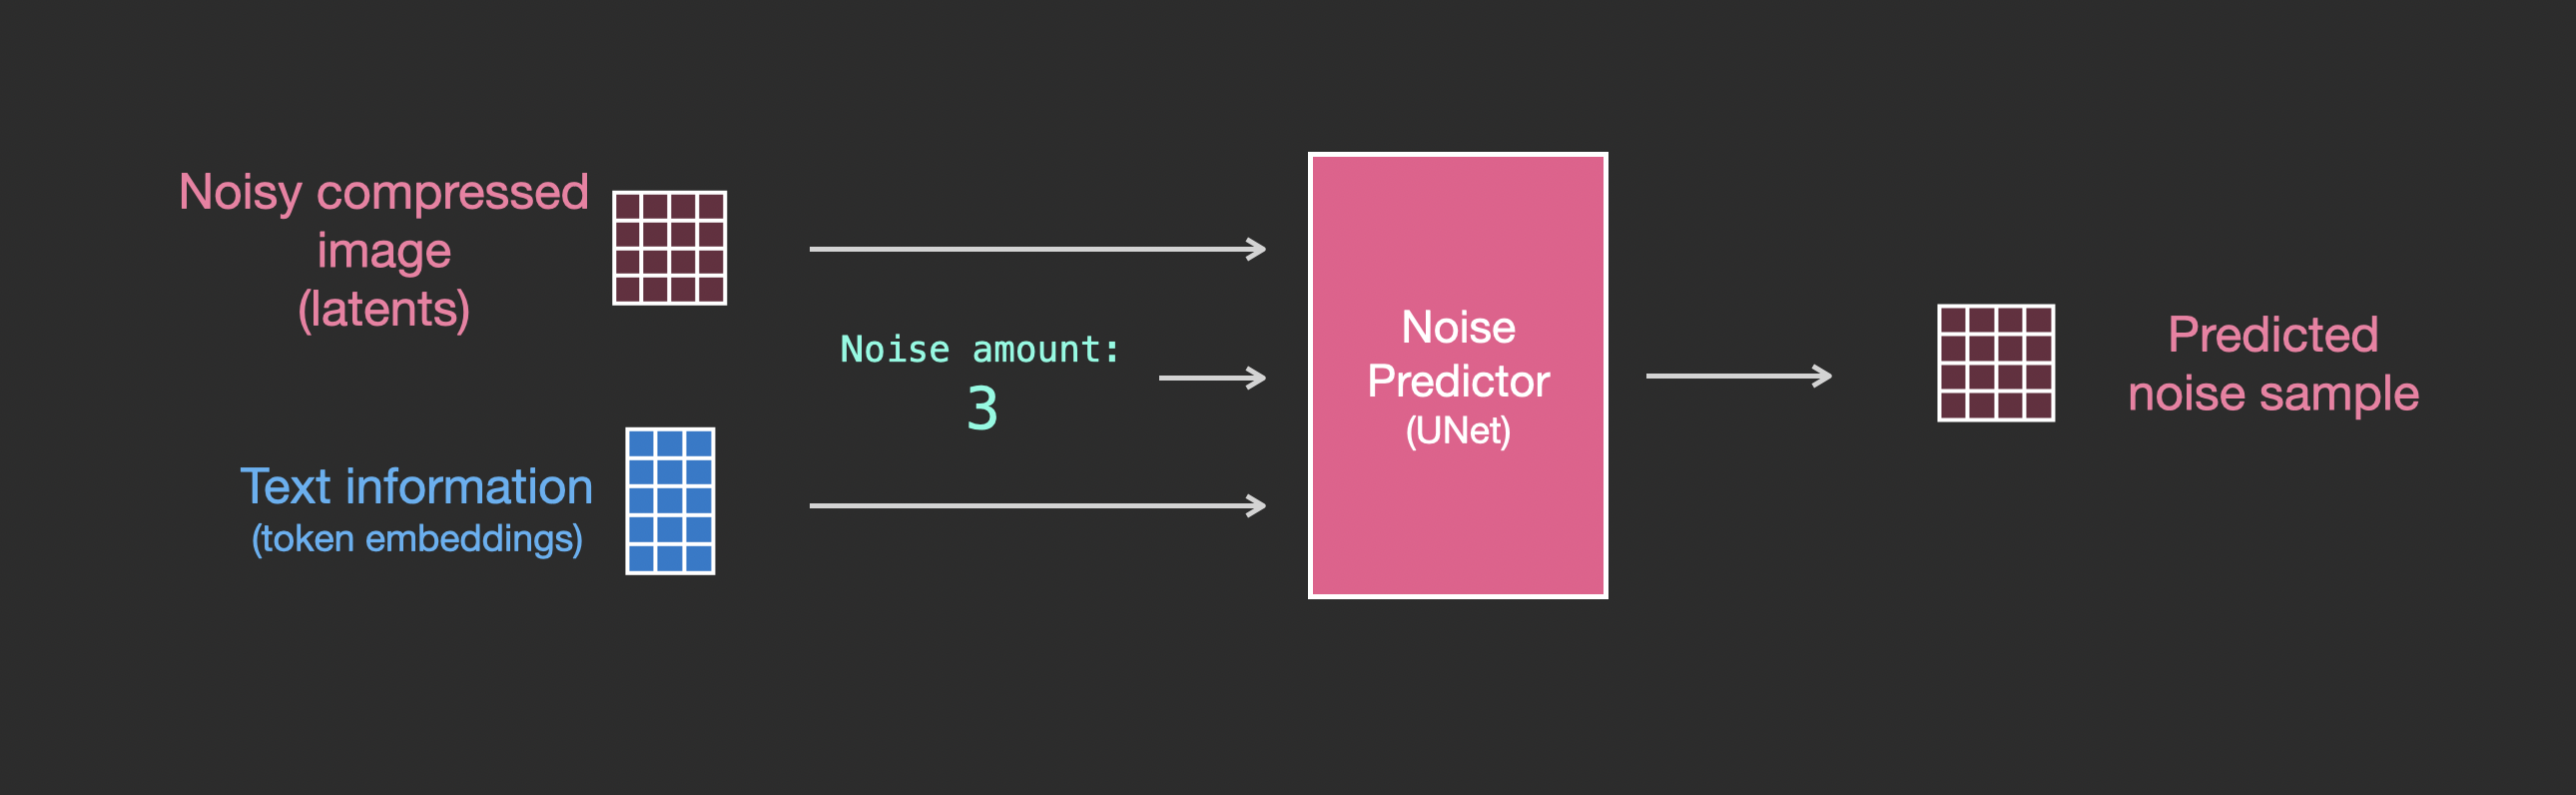
\includegraphics[width=0.95\textwidth]{images/ldm_unet_text.png}
    \captionof{figure}{U-Net (Noise Predictor) nhận ba đầu vào: latent nhiễu ($64\times64\times4$), bước thời gian (noise amount), và text token embeddings ($77\times768$). Xuất ra predicted noise sample cùng kích thước với latent đầu vào.}
    \label{fig:ldm_unet_inputs}
\end{center}

\begin{enumerate}
    \item \textbf{Noisy latent} $\mathbf{z}_t \in \mathbb{R}^{64 \times 64 \times 4}$: latent ở bước $t$ (đang chứa nhiễu).
    \item \textbf{Timestep} $t$: bước thời gian hiện tại (encoded bằng sinusoidal embedding).
    \item \textbf{Text embedding} $\mathbf{c} \in \mathbb{R}^{77 \times 768}$: từ CLIP text encoder.
\end{enumerate}

\textbf{Cross-Attention --- Cơ chế kết nối text và ảnh.}
Text embedding $\mathbf{c}$ được tích hợp vào U-Net qua các lớp \textbf{cross-attention} xen kẽ giữa các ResNet block. Tại mỗi lớp attention:

\[
    \text{Attention}(\mathbf{Q}, \mathbf{K}, \mathbf{V}) = \text{softmax}\!\left(\frac{\mathbf{Q}\mathbf{K}^\top}{\sqrt{d}}\right)\mathbf{V}
\]

\begin{itemize}
    \item $\mathbf{Q}$ (Query) đến từ \textit{latent features} --- ``ảnh đang hỏi: tôi cần thông tin gì từ prompt?''
    \item $\mathbf{K}, \mathbf{V}$ (Key, Value) đến từ \textit{text embedding} $\mathbf{c}$ --- ``prompt trả lời: đây là thông tin tôi có.''
\end{itemize}

Nhờ đó, ở mỗi vị trí không gian trong latent, U-Net ``hỏi'' text embedding xem token nào liên quan nhất đến vùng đó và điều chỉnh denoising cho phù hợp. Ví dụ: khi xử lý vùng latent tương ứng với bầu trời, attention cao vào token ``blue sky''; khi xử lý vùng tiền cảnh, attention cao vào token mô tả vật thể chính.

\begin{center}
    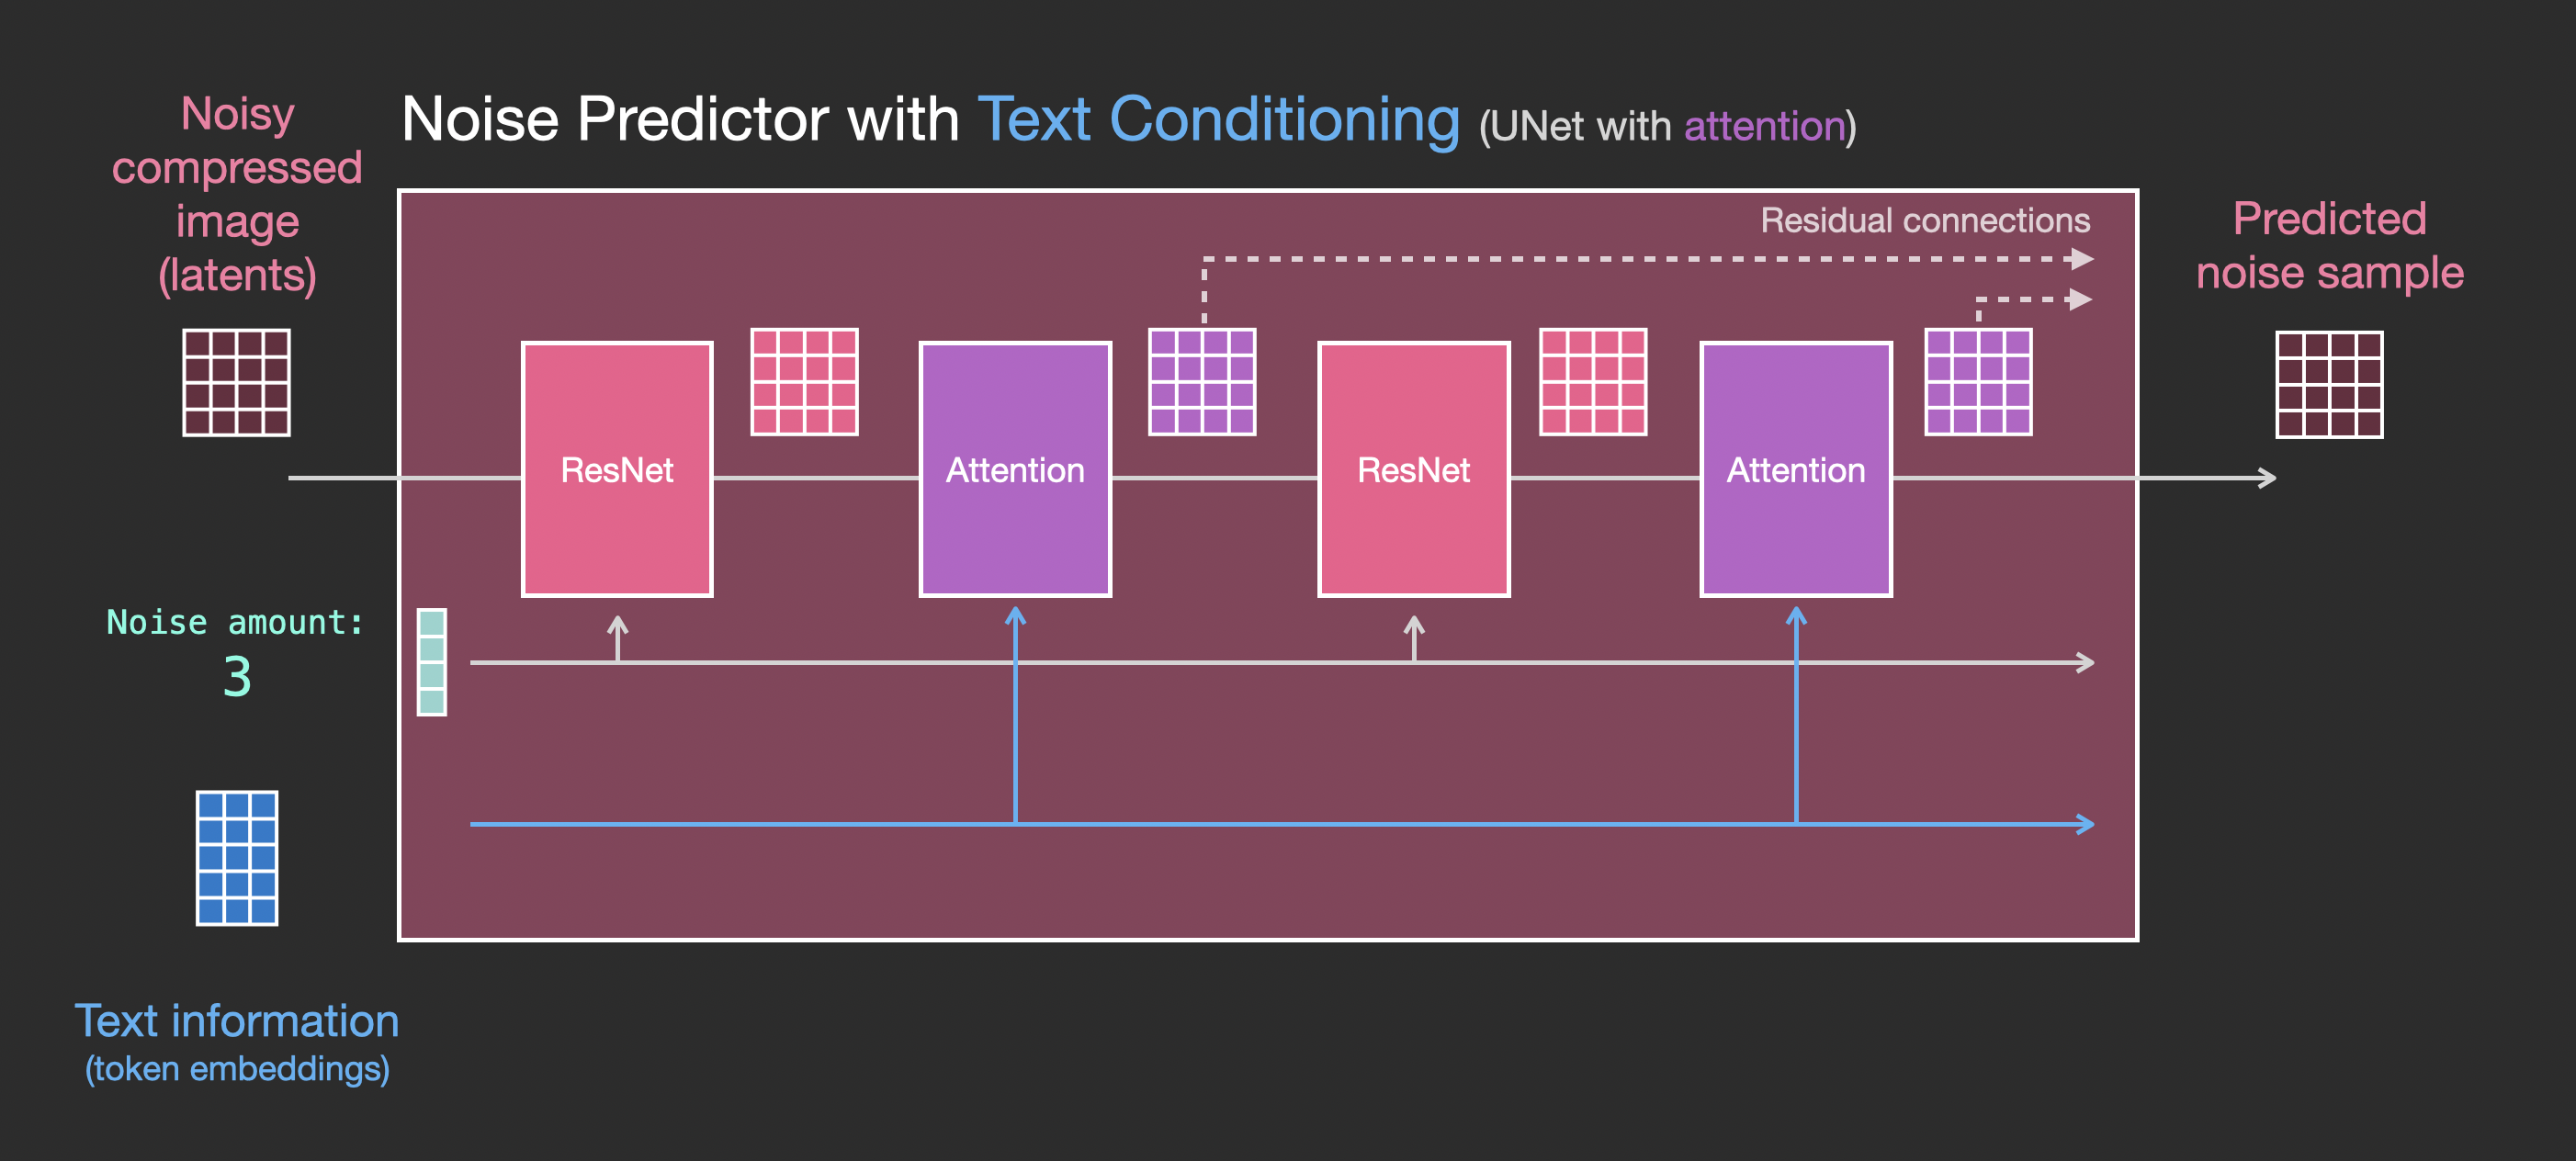
\includegraphics[width=0.98\textwidth]{images/ldm_unet_steps.png}
    \captionof{figure}{Kiến trúc U-Net với text conditioning: xen kẽ ResNet blocks (xử lý không gian) và Attention blocks (kết hợp text qua cross-attention). Text information được inject ở mỗi Attention block, đảm bảo hướng dẫn sinh ảnh xuyên suốt từ encoder đến decoder.}
    \label{fig:ldm_unet_text}
\end{center}

\subsubsection{Pipeline hoàn chỉnh: Từ Văn bản đến Ảnh}

Khi nhận prompt \textit{``a majestic lion at sunset, oil painting style''}:

\begin{center}
    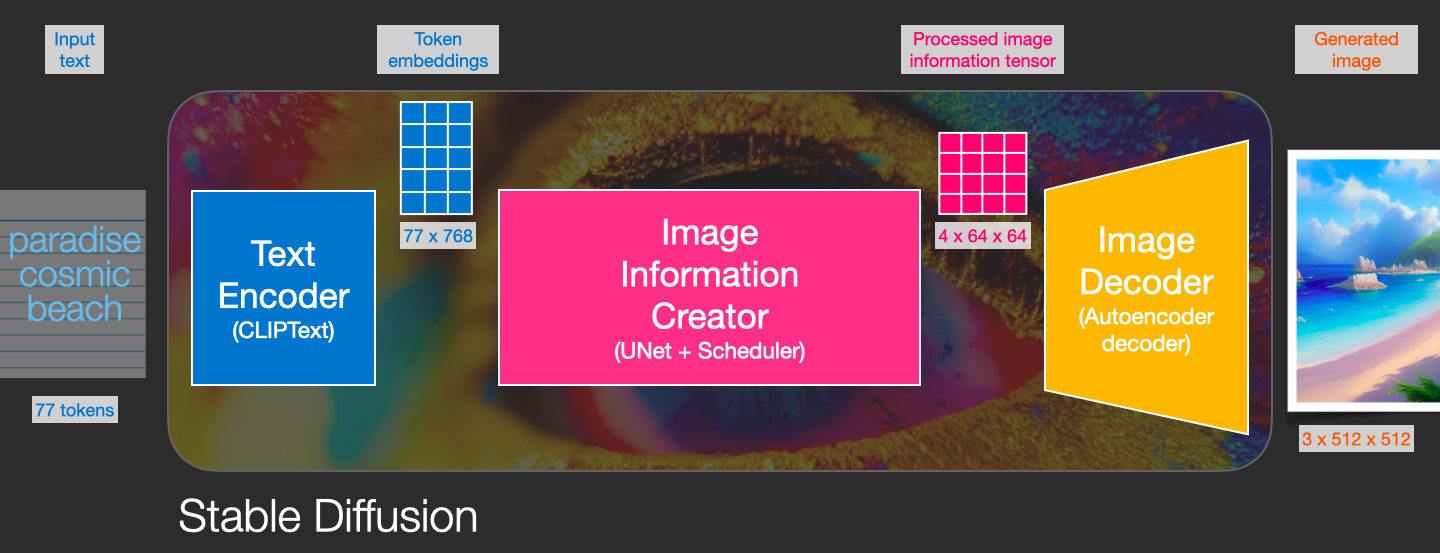
\includegraphics[width=0.95\textwidth]{images/ldm_tensors.png}
    \captionof{figure}{Pipeline đầy đủ với kích thước tensor cụ thể: text prompt → 77 token × 768 chiều; latent nhiễu ban đầu $4\times64\times64$; sau 50 bước denoising với U-Net → latent sạch $4\times64\times64$; VAE decoder → ảnh $512\times512\times3$.}
    \label{fig:ldm_full_pipeline}
\end{center}

\begin{enumerate}
    \item \textbf{Encode text}: CLIP text encoder chuyển prompt thành $\mathbf{c} \in \mathbb{R}^{77 \times 768}$.
    \item \textbf{Khởi tạo}: Lấy mẫu latent nhiễu ngẫu nhiên $\mathbf{z}_T \sim \mathcal{N}(\mathbf{0}, \mathbf{I})$, kích thước $4 \times 64 \times 64$.
    \item \textbf{Denoising loop} ($T = 50$--$100$ bước với DDIM scheduler):
    \begin{itemize}
        \item U-Net dự đoán nhiễu: $\hat{\boldsymbol{\epsilon}} = \boldsymbol{\epsilon}_\theta(\mathbf{z}_t, t, \mathbf{c})$
        \item Áp dụng CFG: kết hợp dự đoán có/không prompt với guidance scale $w$
        \item Tính $\mathbf{z}_{t-1}$ bằng cách trừ nhiễu dự đoán
    \end{itemize}
    \item \textbf{Decode}: VAE decoder chuyển latent sạch $\mathbf{z}_0 \in \mathbb{R}^{4 \times 64 \times 64}$ thành ảnh $\hat{\mathbf{x}} \in \mathbb{R}^{512 \times 512 \times 3}$.
\end{enumerate}

\begin{center}
    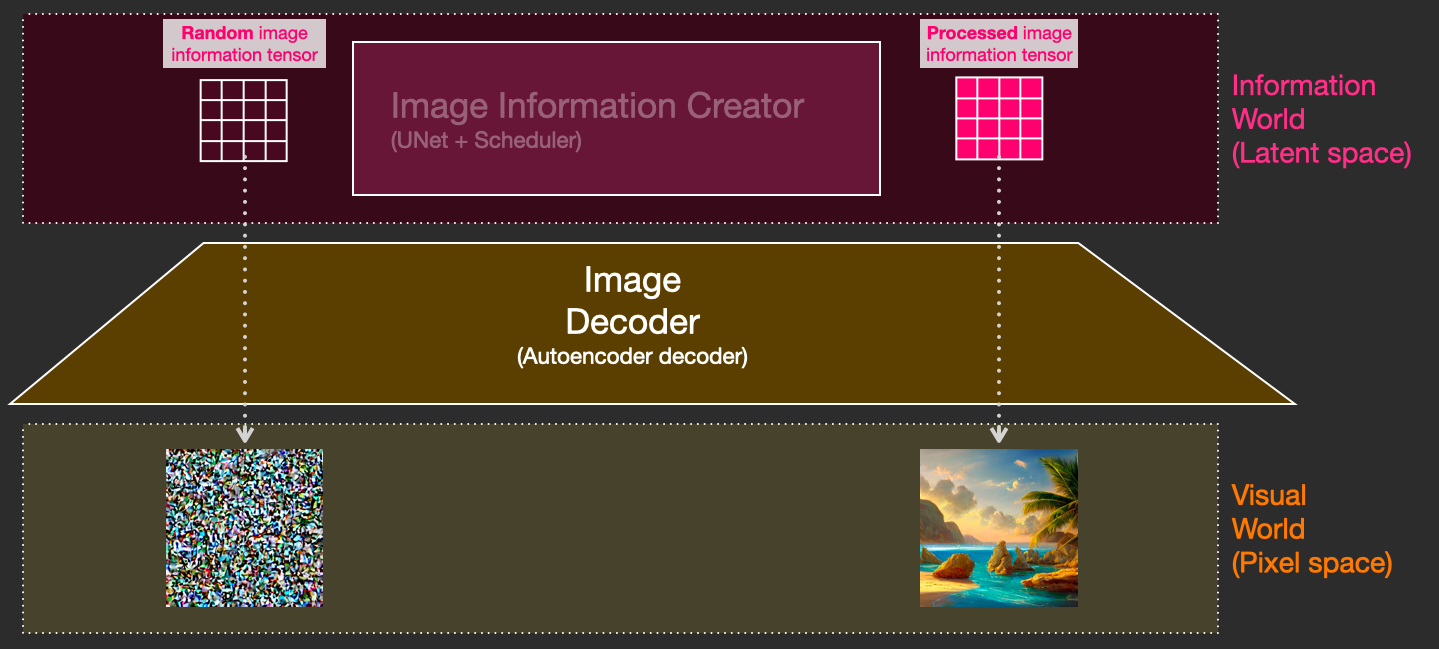
\includegraphics[width=0.90\textwidth]{images/ldm_latent_vs_pixel.png}
    \captionof{figure}{Hai thế giới trong Stable Diffusion: \textbf{Information World} (latent space) nơi U-Net làm việc với tensor nhỏ $4\times64\times64$, và \textbf{Visual World} (pixel space) nơi con người nhìn thấy ảnh $512\times512$. VAE Decoder là cầu nối duy nhất từ latent xuống pixel.}
    \label{fig:ldm_two_worlds}
\end{center}

\textbf{Stable Diffusion} (Rombach et al., 2022) là phiên bản LDM được huấn luyện trên \textbf{LAION-5B} --- bộ dữ liệu 5.8 tỷ cặp ảnh-văn bản thu thập từ internet. Điểm đặc biệt: được phát hành \textbf{mã nguồn mở} với trọng số công khai, tạo ra cả một hệ sinh thái cộng đồng khổng lồ (Civitai, HuggingFace, ComfyUI...). Các phiên bản tiếp theo như \textbf{SDXL} (2023) nâng độ phân giải lên $1024 \times 1024$ và cải thiện chất lượng đáng kể; \textbf{SD 3.0} (2024) dùng kiến trúc Diffusion Transformer thay thế U-Net.

\begin{mdframed}[style=infobox]
\textbf{Tại sao Stable Diffusion nhanh hơn DALL-E hay Midjourney thế hệ đầu?}

DALL-E v1 (OpenAI, 2021) dùng VQ-VAE + Transformer trên token rời rạc --- chậm và giới hạn độ phân giải. Midjourney v1 dùng pixel-space diffusion. Stable Diffusion thực hiện tất cả denoising trong latent $64\times64$ thay vì pixel $512\times512$ --- tức là mỗi bước U-Net nhanh hơn \textbf{48 lần}. Với 50 bước DDIM thay vì 1000 bước DDPM, tổng tốc độ tăng gấp hàng nghìn lần so với DDPM pixel-space gốc. Đây là lý do Stable Diffusion có thể chạy trên laptop consumer GPU 8GB VRAM.
\end{mdframed}
\subsection{Flow Matching: Thế hệ Tiếp theo của Generative Models}
\label{subsec:flow_matching}

Stable Diffusion đã đặt nền tảng vững chắc. Nhưng cộng đồng nghiên cứu tiếp tục đặt câu hỏi: \textit{DDPM có phải cách tốt nhất để vận chuyển từ noise đến data không?} Năm 2022, Lipman et al. \cite{Lipman2022} đề xuất \textbf{Flow Matching} --- một framework hoàn toàn mới, đơn giản hơn, nhanh hơn, và hiệu quả hơn. Đây là nền tảng của \textbf{Stable Diffusion 3} và \textbf{FLUX.1} --- các model sinh ảnh tốt nhất hiện tại.

\subsubsection{Vấn đề với DDPM: Đường cong phức tạp}

DDPM định nghĩa forward process là một \textbf{SDE} (Stochastic Differential Equation) --- phương trình vi phân có yếu tố ngẫu nhiên. Hệ quả là:
\begin{itemize}
    \item Trajectory từ noise $\mathbf{x}_T$ đến data $\mathbf{x}_0$ là \textit{đường cong ngẫu nhiên, phức tạp}, không thể rút ngắn mà không mất chất lượng.
    \item Cần 1000 bước để đi theo đường cong này đủ chính xác.
    \item Noise schedule $\beta_t$ phải được thiết kế cẩn thận; sai schedule có thể làm sụp đổ training.
\end{itemize}

\subsubsection{Ý tưởng cốt lõi: Học Vector Field, đi theo ODE}

Flow Matching tiếp cận bài toán từ góc độ hoàn toàn khác. Thay vì mô hình hóa một SDE ngẫu nhiên, nó học một \textbf{vector field} $v_\theta(\mathbf{x}, t)$ --- một hàm gán cho mỗi điểm $\mathbf{x}$ ở thời điểm $t$ một \textit{hướng di chuyển}. Quá trình sinh ảnh là giải một \textbf{ODE} (Ordinary Differential Equation) đơn giản:

\begin{equation}
    \frac{d\mathbf{x}}{dt} = v_\theta(\mathbf{x}_t, t), \qquad \mathbf{x}_1 \sim \mathcal{N}(\mathbf{0}, \mathbf{I})
    \label{eq:fm_ode}
\end{equation}

\textbf{Đọc phương trình (\ref{eq:fm_ode}):} ``Tốc độ thay đổi của $\mathbf{x}$ tại thời điểm $t$ bằng vector field tại $(\mathbf{x}_t, t)$.'' Bắt đầu từ $\mathbf{x}_1$ (noise thuần túy ở $t=1$), chạy ODE ngược từ $t=1$ về $t=0$ để ra data $\mathbf{x}_0$.

Vì đây là ODE (không có yếu tố ngẫu nhiên trong inference), trajectory \textit{có thể được làm thẳng} --- và đường thẳng thì cần ít bước hơn để đi từ đầu đến cuối.

\begin{center}
    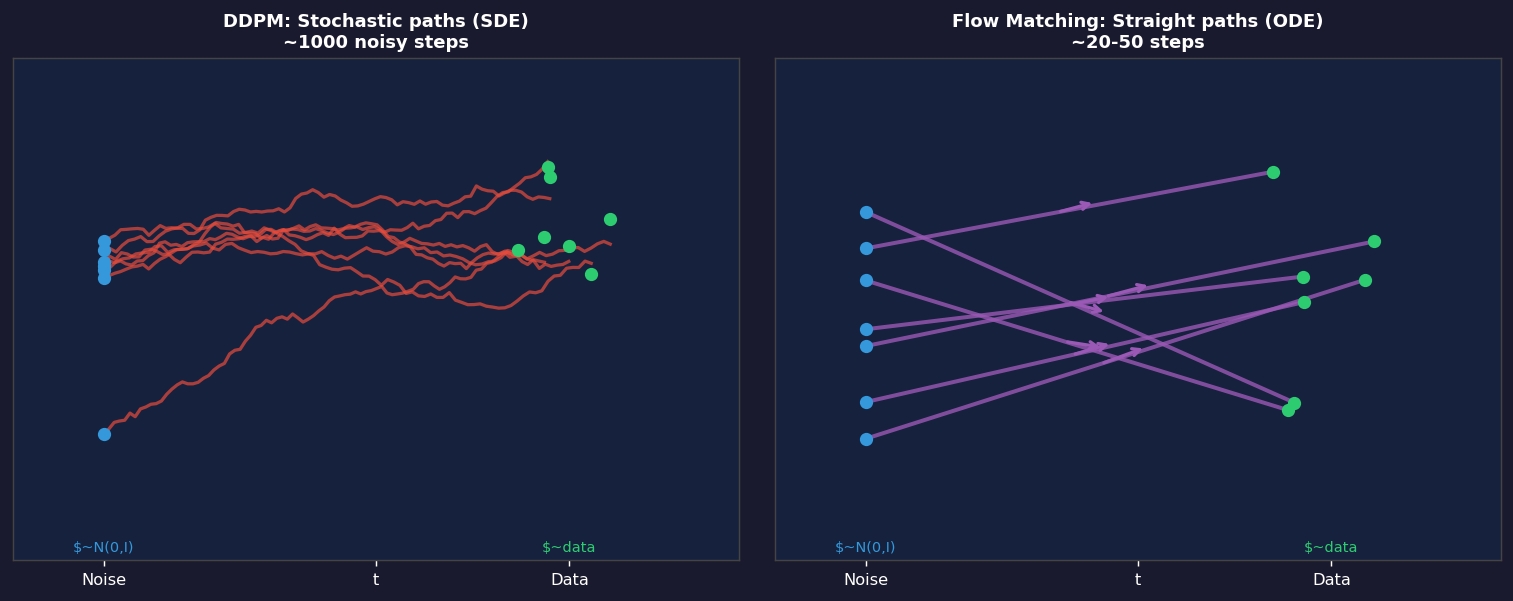
\includegraphics[width=0.95\textwidth]{images/flow_matching_vs_ddpm.png}
    \captionof{figure}{So sánh trajectory từ noise đến data. \textbf{Trái (DDPM)}: đường cong ngẫu nhiên phức tạp (SDE), cần $\sim$1000 bước. \textbf{Phải (Flow Matching)}: đường gần thẳng (ODE), chỉ cần 20--50 bước với chất lượng tương đương hoặc tốt hơn.}
    \label{fig:fm_vs_ddpm}
\end{center}

\subsubsection{Conditional Flow Matching --- Cách train thực tế}

Ta không thể trực tiếp học vector field của toàn bộ phân phối dữ liệu (quá phức tạp). Giải pháp: \textbf{Conditional Flow Matching (CFM)} --- định nghĩa flow cho từng cặp data point riêng lẻ, rồi lấy trung bình.

\textbf{Linear interpolation path.}
Cách đơn giản nhất để kết nối noise $\mathbf{x}_1 \sim \mathcal{N}(\mathbf{0}, \mathbf{I})$ với data $\mathbf{x}_0$: đường thẳng. Điểm trung gian ở thời điểm $t \in [0,1]$:
\begin{equation}
    \mathbf{x}_t = (1 - t)\,\mathbf{x}_0 + t\,\mathbf{x}_1
    \label{eq:fm_interpolation}
\end{equation}
\textbf{Đọc công thức (\ref{eq:fm_interpolation}):} khi $t=0$: $\mathbf{x}_t = \mathbf{x}_0$ (data sạch). Khi $t=1$: $\mathbf{x}_t = \mathbf{x}_1$ (noise thuần túy). Trung gian: mix tuyến tính. Đây là ``Optimal Transport interpolation'' --- đường thẳng là đường ngắn nhất giữa hai điểm.

\textbf{Target vector field.}
Từ phương trình (\ref{eq:fm_interpolation}), vector field ``đúng'' tại mỗi điểm là đạo hàm theo $t$:
\begin{equation}
    u_t(\mathbf{x}_t \mid \mathbf{x}_0) = \frac{d\mathbf{x}_t}{dt} = \mathbf{x}_0 - \mathbf{x}_1
    \label{eq:fm_target}
\end{equation}
\textbf{Điều kỳ diệu}: vector field $u_t = \mathbf{x}_0 - \mathbf{x}_1$ là \textit{hằng số theo $t$} --- không phụ thuộc bước thời gian! Với mỗi cặp $(\mathbf{x}_0, \mathbf{x}_1)$, vector field là cùng một vector từ đầu đến cuối. Điều này giải thích tại sao trajectory là đường thẳng.

\textbf{Training loss.}
Huấn luyện mạng $v_\theta$ để khớp vector field mục tiêu:
\begin{equation}
    \mathcal{L}_{\text{FM}} = \mathbb{E}_{t \sim \mathcal{U}[0,1],\; \mathbf{x}_0 \sim p_\text{data},\; \mathbf{x}_1 \sim \mathcal{N}(\mathbf{0},\mathbf{I})}
    \Bigl[\,\bigl\|v_\theta(\mathbf{x}_t, t) - (\mathbf{x}_0 - \mathbf{x}_1)\bigr\|^2\,\Bigr]
\end{equation}

\textbf{Giải thích từng ký hiệu:}
\begin{itemize}
    \item $t \sim \mathcal{U}[0,1]$: chọn ngẫu nhiên đều một bước thời gian trong $[0,1]$.
    \item $\mathbf{x}_0 \sim p_\text{data}$: lấy một ảnh sạch từ dataset.
    \item $\mathbf{x}_1 \sim \mathcal{N}(\mathbf{0},\mathbf{I})$: lấy một noise vector.
    \item $\mathbf{x}_t = (1-t)\mathbf{x}_0 + t\mathbf{x}_1$: tính điểm trung gian theo (\ref{eq:fm_interpolation}).
    \item $v_\theta(\mathbf{x}_t, t)$: mạng dự đoán vector field tại $(\mathbf{x}_t, t)$.
    \item $\mathbf{x}_0 - \mathbf{x}_1$: target --- vector từ noise về data (hằng số!).
\end{itemize}

Vòng lặp training một bước: (1) lấy $\mathbf{x}_0$ từ dataset và $\mathbf{x}_1$ từ Gaussian, (2) chọn $t$ ngẫu nhiên, (3) tính $\mathbf{x}_t$, (4) mạng dự đoán vector field, (5) MSE loss so với target $\mathbf{x}_0 - \mathbf{x}_1$.

\textbf{Inference.}
Bắt đầu từ noise $\mathbf{x}_1 \sim \mathcal{N}(\mathbf{0}, \mathbf{I})$, giải ODE ngược từ $t=1$ về $t=0$ bằng ODE solver (Euler, RK4, ...):
\[
    \mathbf{x}_{t-\Delta t} = \mathbf{x}_t - \Delta t \cdot v_\theta(\mathbf{x}_t, t)
\]
Với trajectory gần thẳng, bước $\Delta t$ lớn vẫn cho xấp xỉ tốt --- lý do FM chỉ cần 20--50 bước thay vì 1000.

\subsubsection{Kết nối với DDPM và Stable Diffusion}

Nghiên cứu gần đây (xem \cite{Lipman2022} và diffusionflow.github.io) cho thấy DDPM và Gaussian Flow Matching \textit{tương đương toán học} khi dùng cosine schedule và v-prediction. Sự khác biệt không phải ở bản chất mà ở \textit{tham số hóa} và \textit{sampling schedule}:
\begin{itemize}
    \item DDPM tham số hóa qua $\boldsymbol{\epsilon}$ (predict noise) hoặc $\mathbf{x}_0$ (predict clean image).
    \item Flow Matching tham số hóa qua $v$ (predict velocity $= \mathbf{x}_0 - \mathbf{x}_1$).
    \item V-prediction trong DDPM (dùng trong DDIM) thực chất \textit{là} Flow Matching vector field với cosine schedule!
\end{itemize}

\begin{mdframed}[style=infobox]
\textbf{Flow Matching trong thực tế: SD3 và FLUX.1}

\textbf{Stable Diffusion 3} (2024): Rombach et al. kết hợp Flow Matching với kiến trúc \textbf{Multimodal Diffusion Transformer (MMDiT)} --- thay U-Net bằng Transformer xử lý đồng thời text tokens và image tokens trong cùng một attention layer. Kết quả: sinh ảnh chất lượng cao hơn SD2, đặc biệt về text rendering trong ảnh.

\textbf{FLUX.1} (2024, Black Forest Labs): Hiện là model open-source tốt nhất, vượt Midjourney v6 trong nhiều benchmark. Kết hợp Flow Matching + Transformer architecture + Rotary Position Embedding. Có ba phiên bản: FLUX.1-dev (non-commercial), FLUX.1-schnell (distilled, 4 bước), FLUX.1-pro (API).

\textbf{Tại sao Flow Matching thắng?}
\begin{itemize}
    \item Trajectory thẳng hơn → ODE solver cần ít bước hơn → nhanh hơn.
    \item Training loss đơn giản, gradient ổn định hơn (target không thay đổi theo $t$).
    \item Dễ kết hợp với Optimal Transport → phân phối dữ liệu được học hiệu quả hơn.
    \item Tự nhiên mở rộng sang video, 3D, protein folding (AlphaFold 3 dùng Flow Matching!).
\end{itemize}
\end{mdframed}

\subsection{Kỹ thuật Điều khiển Quá trình Sinh ảnh}
\label{subsec:diffusion_control_techniques}

Sức mạnh thực sự của các mô hình khuếch tán không chỉ nằm ở khả năng tạo ra các ảnh ngẫu nhiên chất lượng cao, mà còn ở khả năng kiểm soát và tùy chỉnh quá trình sinh một cách tinh vi. Nhiều kỹ thuật gần đây cho phép chúng ta điều khiển nội dung, bố cục, phong cách, và thậm chí là các đối tượng cụ thể trong ảnh.

\begin{description}
	\item[Textual Inversion:] \cite{Gal2022_textual} 
	\begin{itemize}
		\item \textbf{Mục tiêu:} Cho phép mô hình học một khái niệm thị giác mới từ chỉ một vài (3-5) bức ảnh, mà không cần huấn luyện lại toàn bộ mô hình.
		\item \textbf{Cơ chế:} 
		\begin{enumerate}
			\item Giữ "đóng băng" toàn bộ mô hình diffusion và text encoder.
			\item Tối ưu hóa một embedding vector mới trong từ vựng của text encoder, ví dụ `S*`.
			\item Vector `S*` có thể được dùng trong prompt như một từ khóa: \textit{"a photo of S* in the style of Van Gogh"}.
		\end{enumerate}
		\item \textbf{Ưu điểm:} Nhanh, tiết kiệm tài nguyên, dễ tích hợp vào pipeline hiện có.
		\item \textbf{Hạn chế:} Khả năng tạo ra các chi tiết phức tạp hoặc phong cách đặc trưng đôi khi kém hơn các phương pháp fine-tune.
	\end{itemize}
	
	\item[DreamBooth:] \cite{Ruiz2023_dreambooth}
	\begin{itemize}
		\item \textbf{Mục tiêu:} Cá nhân hóa mô hình diffusion để sinh ra các đối tượng hoặc phong cách cụ thể với độ chính xác cao.
		\item \textbf{Cơ chế:} 
		\begin{enumerate}
			\item Thay vì chỉ học một embedding, DreamBooth tinh chỉnh một phần nhỏ của toàn bộ U-Net.
			\item Sử dụng một định danh lớp hiếm (rare class token), ví dụ `sks`, để tránh quên các khái niệm gốc: \textit{"a photo of a sks dog"}.
			\item Kết hợp dữ liệu ảnh mới của đối tượng với prompt để mô hình học cả nội dung và phong cách đặc trưng.
		\end{enumerate}
		\item \textbf{Ưu điểm:} Tạo ảnh cá nhân hóa rất chính xác, duy trì các chi tiết đặc trưng của đối tượng.
		\item \textbf{Hạn chế:} Yêu cầu nhiều tài nguyên hơn so với Textual Inversion và quá trình fine-tune cần cẩn trọng để tránh "overfitting".
	\end{itemize}
	
	\item[ControlNet:] \cite{Zhang2023_controlnet}
	\begin{itemize}
		\item \textbf{Mục tiêu:} Tăng khả năng điều khiển chi tiết quá trình sinh ảnh bằng các điều kiện không gian như đường viền (edges), tư thế (pose), độ sâu (depth map) hoặc phác thảo (scribbles).
		\item \textbf{Kiến trúc:} 
		\begin{enumerate}
			\item Đóng băng toàn bộ mô hình diffusion lớn đã được huấn luyện trước (như Stable Diffusion).
			\item Tạo một bản sao của các khối mã hóa trong mô hình gốc và huấn luyện bản sao này (gọi là "ControlNet") để nhận thêm đầu vào điều kiện.
			\item Output từ ControlNet được cộng vào output của các lớp tương ứng trong mô hình diffusion gốc, "hướng dẫn" quá trình khử nhiễu theo cấu trúc mong muốn.
		\end{enumerate}
		\item \textbf{Quá trình hoạt động:} 
		\begin{itemize}
			\item Nhập ảnh điều kiện (ví dụ: skeleton pose, edge map) vào ControlNet.
			\item ControlNet điều chỉnh các đặc trưng trong quá trình diffusion, đảm bảo ảnh sinh ra tuân theo bố cục/chi tiết của điều kiện.
		\end{itemize}
		\item \textbf{Ưu điểm:} 
		\begin{itemize}
			\item Cho phép kiểm soát chính xác bố cục, tư thế, và các chi tiết hình học.
			\item Dễ kết hợp với các kỹ thuật điều kiện khác như Text-to-Image hoặc DreamBooth.
		\end{itemize}
		\item \textbf{Hạn chế:} Yêu cầu ảnh điều kiện phù hợp và đôi khi tăng chi phí tính toán.
	\end{itemize}
\end{description}

\begin{center}
	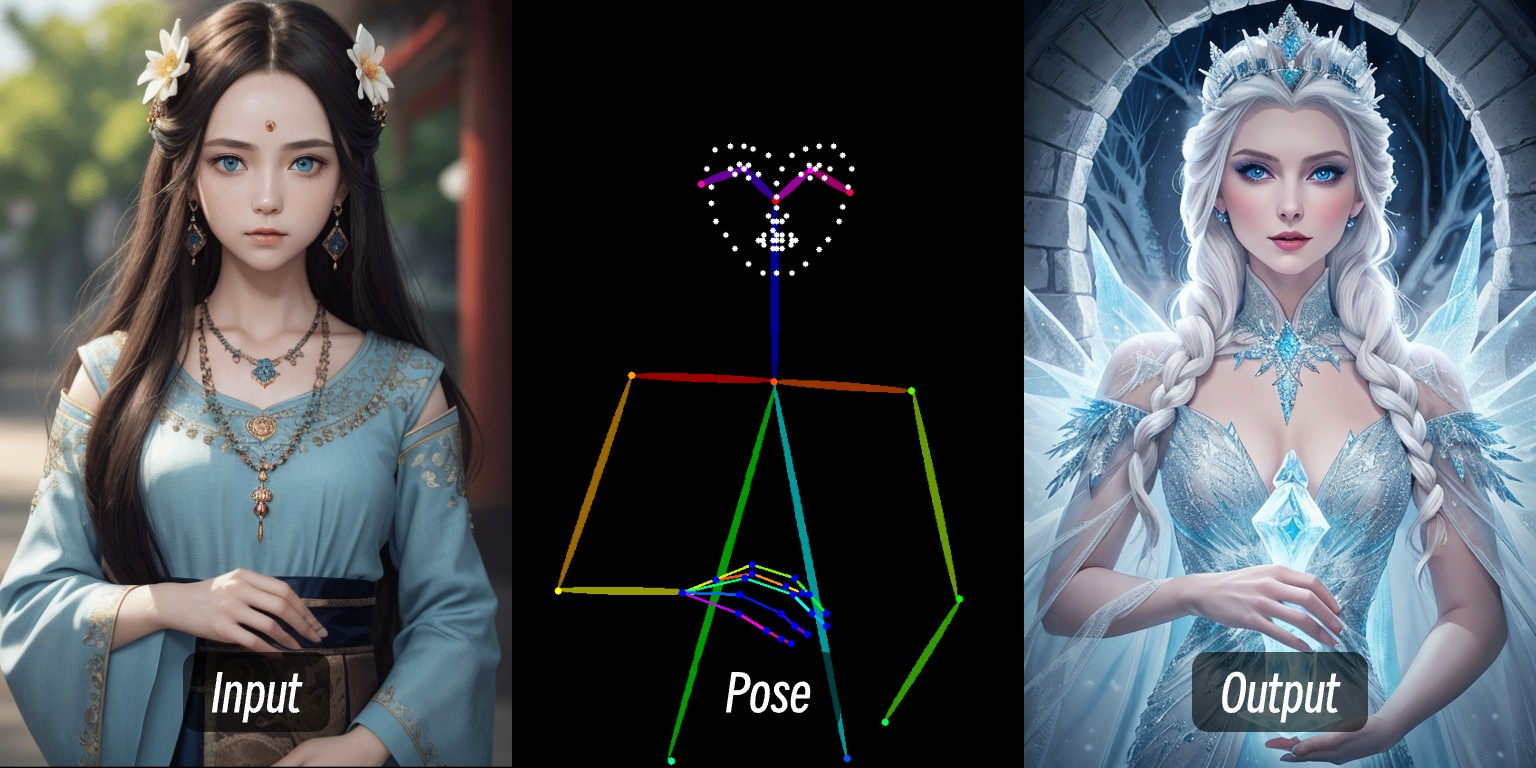
\includegraphics[width=1.0\textwidth]{images/controlnet_pose_example.jpg}
	\captionof{figure}{Ví dụ về ControlNet: bằng cách cung cấp một ảnh tư thế (pose) làm điều kiện, ControlNet hướng dẫn mô hình diffusion (Stable Diffusion) tạo ra nhân vật với tư thế chính xác.}
	\label{fig:controlnet_example}
\end{center}

\subsection{Kết luận: Một Kỷ nguyên Mới của Sáng tạo Thị giác}
\label{subsec:diffusion_conclusion}
Các mô hình khuếch tán đã thay đổi cuộc chơi trong lĩnh vực AI sáng tạo. Chúng không chỉ vượt qua GANs về chất lượng và sự đa dạng của ảnh sinh ra, mà còn cung cấp một nền tảng ổn định và cực kỳ linh hoạt để điều khiển quá trình sáng tạo.

Từ nền tảng lý thuyết của DDPM, sự tối ưu hóa hiệu quả của Latent Diffusion, đến khả năng kiểm soát tinh vi của ControlNet, DreamBooth, và Textual Inversion, các mô hình khuếch tán đã dân chủ hóa khả năng sáng tạo nghệ thuật, biến những ý tưởng trong văn bản thành những tác phẩm thị giác chi tiết. Chúng là công nghệ cốt lõi đằng sau cuộc cách mạng text-to-image và đang nhanh chóng được mở rộng sang các lĩnh vực video, 3D, và âm thanh, hứa hẹn một tương lai nơi ranh giới giữa trí tưởng tượng của con người và khả năng tổng hợp của máy móc ngày càng bị xóa nhòa.

\section*{Tài liệu tham khảo}
\begin{itemize}
	\item[1] Ho, J., Jain, A., \& Abbeel, P. (2020). Denoising diffusion probabilistic models. In \textit{Advances in Neural Information Processing Systems (NeurIPS)}. (Paper gốc giới thiệu DDPM).
	\item[2] Rombach, R., Blattmann, A., Lorenz, D., Esser, P., \& Ommer, B. (2022). High-resolution image synthesis with latent diffusion models. In \textit{Proceedings of the IEEE/CVF Conference on Computer Vision and Pattern Recognition (CVPR)}. (Paper gốc giới thiệu Latent Diffusion Models, nền tảng của Stable Diffusion).
	\item[3] Zhang, L., \& Agrawala, M. (2023). Adding conditional control to text-to-image diffusion models. In \textit{Proceedings of the IEEE/CVF International Conference on Computer Vision (ICCV)}. (Paper gốc giới thiệu ControlNet).
	\item[4] Gal, R., Alaluf, Y., Atzmon, Y., Patashnik, O., Bermano, A. H., \& Cohen-Or, D. (2022). An image is worth one word: Personalizing text-to-image generation using textual inversion. In \textit{ECCV Workshops}. (Paper gốc giới thiệu Textual Inversion).
	\item[5] Ruiz, N., Li, Y., Jampani, V., Pritch, Y., Rubinstein, M., \& Aberman, K. (2023). Dreambooth: Fine-tuning text-to-image diffusion models for subject-driven generation. In \textit{Proceedings of the IEEE/CVF Conference on Computer Vision and Pattern Recognition (CVPR)}. (Paper gốc giới thiệu DreamBooth).
	\item[6] Dhariwal, P., \& Nichol, A. (2021). Diffusion models beat GANs on image synthesis. In \textit{Advances in Neural Information Processing Systems (NeurIPS)}. (Paper giới thiệu Classifier Guidance).
	\item[7] Ho, J., \& Salimans, T. (2022). Classifier-free diffusion guidance. In \textit{NeurIPS Workshop on Deep Generative Models}. (Paper giới thiệu Classifier-Free Guidance - CFG).
	\item[8] Sohl-Dickstein, J., Weiss, E., Maheswaranathan, N., \& Ganguli, S. (2015). Deep unsupervised learning using nonequilibrium thermodynamics. In \textit{International Conference on Machine Learning (ICML)}. (Một trong những công trình lý thuyết sơ khai đặt nền móng cho các mô hình khuếch tán).
\end{itemize}